\chapter*{گزارش کار پروژه}

\section{مقدمه}
\subsection{تحلیل احساسات \lr{(Sentiment Analysis)}}
در سال‌های اخیر، با گسترش اینترنت و توسعه تجارت الکترونیک، حجم عظیمی از داده‌های متنی توسط کاربران در فضای وب تولید شده است. بخش قابل توجهی از این داده‌ها شامل نظرات، پیشنهادها، انتقادات و تجربیات کاربران درباره محصولات و خدمات مختلف است. یکی از مهم‌ترین شاخه‌های پردازش زبان طبیعی \lr{(Natural Language Processing)}، تحلیل احساسات است؛ که به فرآیند شناسایی و طبقه‌بندی احساس موجود در یک متن گفته می‌شود و هدف آن تعیین نگرش نویسنده نسبت به یک موضوع، محصول یا خدمت است. در ساده‌ترین حالت، خروجی این فرآیند شامل سه دسته احساس مثبت، منفی و خنثی خواهد بود. امروزه تحلیل احساسات در حوزه‌های مختلفی از جمله تجارت الکترونیک، شبکه‌های اجتماعی، بازاریابی دیجیتال، سیستم‌های پیشنهاددهنده و تحلیل بازخورد مشتریان کاربرد گسترده‌ای پیدا کرده است و نقش مهمی در استخراج دانش از داده‌های متنی ایفا می‌کند.

\subsection{اهمیت تحلیل نظرات کاربران}
نظرات کاربران یکی از مهم‌ترین منابع اطلاعاتی برای ارزیابی کیفیت محصولات و خدمات محسوب می‌شوند. کاربران معمولاً پس از خرید، تجربه واقعی خود را در قالب متن، امتیازدهی و پیشنهاد یا عدم پیشنهاد محصول ثبت می‌کنند. این اطلاعات می‌تواند دیدگاه جامعی درباره نقاط قوت و ضعف یک محصول در اختیار خریداران آینده و همچنین تولیدکنندگان قرار دهد. با توجه به حجم بسیار زیاد این نظرات، بررسی دستی آن‌ها عملاً امکان‌پذیر نیست؛ بنابراین استفاده از روش‌های خودکار مبتنی بر یادگیری ماشین و پردازش زبان طبیعی به کسب‌وکارها کمک می‌کند تا در مدت زمان کوتاهی حجم عظیمی از داده‌های متنی را تحلیل کرده و اطلاعات ارزشمندی برای تصمیم‌گیری، بهبود کیفیت محصولات و افزایش رضایت مشتریان کسب کنند.

\subsection{دلیل انتخاب دیجی‌کالا}
در این پروژه، داده‌های فروشگاه اینترنتی دیجی‌کالا به‌عنوان منبع اصلی اطلاعات انتخاب شده‌اند. دیجی‌کالا یکی از بزرگ‌ترین فروشگاه‌های اینترنتی ایران است که میلیون‌ها کاربر فعال داشته و روزانه تعداد زیادی نظر درباره محصولات مختلف در آن ثبت می‌شود. این مجموعه داده علاوه بر متن نظرات، اطلاعات ارزشمند دیگری نظیر امتیاز کاربران، وضعیت پیشنهاد خرید، تعداد لایک و دیسلایک، اطلاعات محصول، برند، قیمت و سایر مشخصات را نیز در اختیار قرار می‌دهد. تنوع بالای محصولات، حجم زیاد داده‌ها و فارسی بودن متون، این مجموعه را به گزینه‌ای مناسب برای طراحی و ارزیابی یک سامانه تحلیل احساسات زبان فارسی تبدیل کرده است.
\subsection{هدف پروژه}
هدف اصلی این پروژه، طراحی و پیاده‌سازی یک سامانه جامع تحلیل احساسات برای نظرات فارسی کاربران دیجی‌کالا است که بتواند با استفاده از تکنیک‌های پردازش زبان طبیعی و الگوریتم‌های یادگیری ماشین، احساس هر نظر را به‌صورت خودکار در یکی از سه دسته مثبت، منفی یا خنثی طبقه‌بندی کند. برای تحقق این هدف، ابتدا داده‌های مربوط به محصولات و نظرات کاربران جمع‌آوری و پیش‌پردازش شده‌اند، سپس ویژگی‌های مناسب از داده‌ها استخراج و چندین مدل یادگیری ماشین آموزش و ارزیابی شده‌اند تا بهترین مدل انتخاب شود. علاوه بر بخش هوش مصنوعی، یک سامانه نرم‌افزاری کامل شامل Backend مبتنی بر FastAPI ، پایگاه داده SQLite و رابط کاربری تحت وب (Frontend) نیز توسعه یافته است تا کاربران بتوانند به‌صورت تعاملی نظرات را تحلیل کرده، نتایج را مشاهده کنند، تاریخچه تحلیل‌ها را مدیریت نمایند و اطلاعات تحلیلی مربوط به محصولات را دریافت کنند. در نتیجه، این پروژه یک سامانه End-to-End را از مرحله آماده‌سازی داده‌ها تا ارائه سرویس و نمایش نتایج به کاربران پیاده‌سازی می‌کند و قابلیت توسعه برای استفاده در مقیاس‌های بزرگ‌تر را نیز داراست.


\section{تعریف مسئله}
\subsection{مسئله‌ای که پروژه حل می‌کند}
با رشد روزافزون فروشگاه‌های اینترنتی، تعداد نظرات ثبت‌شده توسط کاربران درباره محصولات نیز به شکل قابل توجهی افزایش یافته است. این نظرات حاوی اطلاعات ارزشمندی درباره کیفیت محصولات، میزان رضایت مشتریان، نقاط قوت و نقاط ضعف آن‌ها هستند. با این حال، حجم بالای داده‌های متنی باعث می‌شود بررسی و تحلیل دستی آن‌ها بسیار زمان‌بر، پرهزینه و در بسیاری از موارد غیرممکن باشد. از سوی دیگر، تصمیم‌گیری تنها بر اساس امتیاز عددی محصولات نمی‌تواند تصویر کاملی از تجربه کاربران ارائه دهد؛ زیرا ممکن است یک محصول امتیاز بالایی داشته باشد، اما کاربران در نظرات خود به مشکلات خاصی مانند کیفیت ساخت، عملکرد یا خدمات پس از فروش اشاره کرده باشند.

هدف اصلی این پروژه، ارائه یک راهکار هوشمند برای تحلیل خودکار نظرات فارسی کاربران دیجی‌کالا است.
\subsection{ورودی و خروجی سیستم}
ورودی اصلی سیستم، متن نظرات کاربران به زبان فارسی است که می‌تواند به‌صورت یک نظر یا مجموعه‌ای از چندین نظر به سامانه ارسال شود. علاوه بر داده‌های متنی، در مرحله آموزش مدل از اطلاعات تکمیلی موجود در مجموعه داده نظیر امتیاز محصول، وضعیت پیشنهاد خرید، وضعیت خریدار، تعداد واکنش‌های کاربران، اطلاعات قیمتی و مشخصات محصولات نیز برای استخراج ویژگی‌های مؤثر استفاده شده است.

پس از پردازش متن و اعمال مراحل پیش‌پردازش، مدل آموزش‌دیده احساس هر نظر را پیش‌بینی می‌کند. خروجی سیستم شامل برچسب احساس (مثبت، منفی یا خنثی)، میزان اطمینان مدل نسبت به پیش‌بینی انجام‌شده \lr{(Confidence Score)} و متن پیش‌پردازش‌شده است. همچنین در بخش جزئیات محصولات، سامانه قادر است خلاصه‌ای از نظرات کاربران، تعداد نظرات هر دسته احساسی و درصد توزیع احساسات مربوط به یک محصول را نیز ارائه دهد.
\subsection{محدودیت‌های پروژه}
با وجود عملکرد مطلوب سامانه، این پروژه با محدودیت‌هایی نیز همراه است. یکی از مهم‌ترین محدودیت‌ها، حجم بسیار زیاد مجموعه داده است. از آنجا که دیتاست اصلی شامل حدود شش میلیون نظر کاربران و بیش از یک میلیون اطلاعات محصول است، آموزش مدل روی کل داده‌ها به منابع پردازشی و حافظه بسیار بالایی نیاز دارد. به همین دلیل، در این پروژه از نمونه‌ای شامل حدود 100 تا 200 هزار رکورد برای آموزش و ارزیابی مدل استفاده شده است.

از سوی دیگر، زبان فارسی دارای ویژگی‌هایی مانند تنوع نگارشی، استفاده از اصطلاحات محاوره‌ای، غلط‌های املایی، شکل‌های مختلف نوشتاری و ابهام‌های معنایی است که فرآیند تحلیل احساسات را با چالش مواجه می‌کند. همچنین، تشخیص دقیق نظرات خنثی نسبت به نظرات مثبت و منفی دشوارتر بوده و این موضوع بر عملکرد مدل تأثیرگذار است. علاوه بر این، مدل پیاده‌سازی‌شده از الگوریتم‌های کلاسیک یادگیری ماشین استفاده می‌کند و هنوز از مدل‌های عمیق مبتنی بر ترنسفورمر مانند ParsBERT بهره نمی‌برد که می‌تواند در آینده موجب بهبود دقت سیستم شود.
\subsection{کاربردهای سیستم}
سامانه توسعه‌یافته می‌تواند در حوزه‌های مختلف تجارت الکترونیک و تحلیل داده‌های متنی مورد استفاده قرار گیرد. فروشگاه‌های اینترنتی قادر خواهند بود با استفاده از این سیستم، میزان رضایت مشتریان از محصولات مختلف را به‌صورت خودکار ارزیابی کرده و نقاط قوت و ضعف محصولات را شناسایی کنند. همچنین تولیدکنندگان و فروشندگان می‌توانند با تحلیل بازخورد مشتریان، کیفیت محصولات و خدمات خود را بهبود دهند.

از سوی دیگر، کاربران نیز می‌توانند پیش از خرید یک محصول، به‌جای مطالعه تعداد زیادی نظر، خلاصه‌ای از دیدگاه سایر خریداران و توزیع احساسات ثبت‌شده را مشاهده کرده و تصمیم آگاهانه‌تری اتخاذ کنند. علاوه بر این، معماری ماژولار پروژه و ارائه سرویس‌های REST API باعث شده است که این سامانه قابلیت استفاده در سایر نرم‌افزارها، وب‌سایت‌ها و سیستم‌های هوشمند را نیز داشته باشد و در آینده بتوان آن را با مدل‌های پیشرفته‌تر، سیستم‌های پیشنهاددهنده محصولات و سایر کاربردهای مبتنی بر هوش مصنوعی توسعه داد.
\section{ابزارها و فناوری‌های استفاده‌شده}
در این پروژه، از مجموعه‌ای از ابزارها و فناوری‌های متن‌باز برای پیاده‌سازی بخش‌های مختلف سیستم شامل پردازش داده، یادگیری ماشین، توسعه Backend ، طراحی Frontend و مدیریت پایگاه داده استفاده شده است. انتخاب این ابزارها با هدف افزایش کارایی، توسعه‌پذیری و سهولت نگهداری سامانه انجام شده است. در ادامه به معرفی و توضیحی کوتاه در موردشان می‌پردازیم.
\subsection{زبان برنامه‌نویسی}
\begin{itemize}
	\item [Python] 
	به‌عنوان هسته اصلی پروژه دارای سادگی، جامعه کاربری گسترده و وجود کتابخانه‌های قدرتمند در حوزه علم داده، یادگیری ماشین و توسعه وب است که این زبان را به یکی از بهترین گزینه‌ها برای پروژه‌های هوش مصنوعی تبدیل کرده است. تمامی مراحل پردازش داده، آموزش مدل، توسعه API و ارتباط با پایگاه داده در این پروژه با استفاده از پایتون انجام شده است.
	\item[TypeScript] 
	از این زبان برای توسعه رابط کاربری پروژه استفاده شده است. زبان تایپ اسکریپت به دلیل مدیریت کامل انواع دیتا تایپ‌ها گزینه بسیار مناسب‌تری نسبت به جاوااسکریپت برای ارتباط با API ها می‌باشد.
\end{itemize}
\subsection{ابزارهای یادگیری ماشین و پردازش داده}
\begin{itemize}
	\item Pandas 
	برای بارگذاری، مدیریت، پاک‌سازی، ادغام و تحلیل داده‌های جدولی مورد استفاده قرار گرفته است. بخش عمده عملیات آماده‌سازی داده‌ها و Feature Engineering با استفاده از این کتابخانه انجام شده است.
	\item NumPy 
	برای انجام محاسبات عددی، عملیات روی آرایه‌ها و افزایش سرعت پردازش داده‌ها مورد استفاده قرار گرفته و پایه بسیاری از محاسبات کتابخانه‌های یادگیری ماشین را تشکیل می‌دهد.
	\item Hazm 
	یکی از مهم‌ترین کتابخانه‌های پردازش زبان طبیعی فارسی است که در این پروژه برای نرمال‌سازی متن، توکن‌سازی، حذف نویسه‌های اضافی و آماده‌سازی نظرات فارسی پیش از آموزش مدل استفاده شده است.
	\item Scikit-Learn 
	این کتابخانه اصلی‌ترین ابزار یادگیری ماشین پروژه محسوب می‌شود. الگوریتم‌های طبقه‌بندی، استخراج ویژگی با TF-IDF ، تقسیم داده‌ها، ارزیابی مدل، تنظیم ابرپارامترها (GridSearchCV) و سایر مراحل آموزش و ارزیابی مدل با استفاده از این کتابخانه انجام شده‌اند.
	\item Joblib 
	برای ذخیره و بارگذاری مدل نهایی آموزش‌دیده و بردارساز TF-IDF از این کتابخانه استفاده شده است. این کار موجب می‌شود مدل تنها یک‌بار آموزش داده شده و در زمان اجرای وب سرویس مستقیماً مورد استفاده قرار گیرد.
	\item Jupyter Notebook 
	فرآیند تحلیل داده‌ها، انجام آزمایش‌های مختلف، آموزش مدل‌ها، مقایسه نتایج و مستندسازی مراحل توسعه در محیط Jupyter Notebook انجام شده است. این محیط امکان اجرای مرحله‌به‌مرحله کد و مشاهده هم‌زمان نتایج را فراهم می‌کند.
\end{itemize}
\subsection{ابزارهای توسعه Backend}
\begin{itemize}
	\item FastAPI
	برای توسعه وب‌سرویس پروژه از این فریم‌ورک استفاده شده است. این فریم‌ورک به دلیل سرعت بالا، پشتیبانی از برنامه‌نویسی ناهمگام \lr{ (Asynchronous Programming)}، تولید خودکار مستندات API ، سادگی در پیاده‌سازی و عملکرد مناسب، انتخاب مناسبی برای ارائه سرویس محسوب می‌شود.
	\item SQLite
	به‌منظور ذخیره تاریخچه تحلیل‌ها و اطلاعات مربوط به محصولات، از این  پایگاه داده استفاده شده است. سبک بودن، عدم نیاز به نصب جداگانه و سادگی مدیریت از مهم‌ترین دلایل انتخاب این پایگاه داده برای پروژه بوده است.
	\item SQLAlchemy 
 به‌عنوان لایه ارتباطی بین برنامه و پایگاه داده مورد استفاده قرار گرفته است. این کتابخانه امکان مدیریت داده‌ها از طریق ORM را فراهم کرده و باعث افزایش خوانایی و قابلیت توسعه کد می‌شود.
\end{itemize}

\subsection{ابزارهای توسعه Frontend}
\begin{itemize}
	\item React
	یک کتابخانه متن‌باز مبتنی بر جاوااسکریپت است که برای طراحی رابط‌های کاربری پویا و تعاملی مورد استفاده قرار می‌گیرد. در این پروژه، React به‌عنوان هسته اصلی Frontend انتخاب شده است. استفاده از معماری مبتنی بر کامپوننت \lr{(Component-Based Architecture)} باعث شده بخش‌های مختلف رابط کاربری به‌صورت مستقل توسعه داده شوند و قابلیت استفاده مجدد از کامپوننت‌ها افزایش یابد.
	\item Tailwind CSS
	یک فریم‌ورک CSS مبتنی بر Utility Classes است که امکان طراحی سریع و منعطف رابط کاربری را فراهم می‌کند. در این پروژه، از Tailwind CSS برای طراحی صفحات، ایجاد چیدمان مناسب، پیاده‌سازی طراحی واکنش‌گرا (Responsive) و یکپارچه‌سازی ظاهر بخش‌های مختلف استفاده شده است.
	\item Zustand
	یک کتابخانه سبک برای مدیریت وضعیت (State Management) در برنامه‌های React است. در این پروژه، از Zustand برای مدیریت داده‌های مشترک بین صفحات مختلف مانند اطلاعات محصولات، نتایج تحلیل احساسات و وضعیت بارگذاری استفاده شده است.
	\item Axios
	یک کتابخانه محبوب برای ارسال درخواست‌های HTTP در برنامه‌های JavaScript و React است. در این پروژه، تمامی ارتباطات میان Frontend و Backend از طریق Axios انجام می‌شود. درخواست‌هایی مانند تحلیل احساسات، جستجوی محصولات، دریافت اطلاعات هر محصول و دریافت خلاصه نظرات با استفاده از این کتابخانه به سرور ارسال می‌شوند.
	\item smart-persian-tools
	این پکیج که توسط خودم توسعه داده شده و برای تبدیل ارقام انگلیسی به فارسی در پروژه مورد استفاده قرار گرفته است.
\end{itemize}

\section{معرفی دیتاست‌ها}
یکی از مهم‌ترین بخش‌های هر پروژه یادگیری ماشین، انتخاب دیتاست مناسب است. کیفیت، حجم و تنوع داده‌ها تأثیر مستقیمی بر عملکرد مدل نهایی دارند. در این پروژه، از دو دیتاست مرتبط با فروشگاه اینترنتی دیجی‌کالا استفاده شده است که شامل اطلاعات محصولات و نظرات ثبت‌شده توسط کاربران می‌باشد. این دو دیتاست پس از انجام عملیات پیش‌پردازش و ادغام، به‌عنوان داده ورودی فرآیند آموزش مدل مورد استفاده قرار گرفته‌اند.
\subsection{دیتاست نظرات کاربران}
دیتاست نظرات شامل حدود ۶ میلیون نظر ثبت‌شده توسط کاربران درباره محصولات مختلف دیجی‌کالا است. هر رکورد بیانگر نظر یک کاربر درباره یک محصول بوده و علاوه بر متن نظر، اطلاعات تکمیلی متعددی نیز در آن وجود دارد. از مهم‌ترین ستون‌های این دیتاست می‌توان به موارد زیر اشاره کرد:
\begin{itemize}
	\item شناسه محصول \lr{(Product ID)}
	\item متن نظر \lr{(Comment Body)}
	\item امتیاز ثبت‌شده توسط کاربر \lr{(Rating)}
	\item وضعیت پیشنهاد خرید \lr{(Recommendation Status)}
	\item وضعیت خریدار \lr{(Verified Buyer)}
	\item تعداد لایک و دیسلایک هر نظر
	\item تاریخ ثبت نظر
\end{itemize}
وجود این اطلاعات باعث می‌شود علاوه بر متن، بتوان از ویژگی‌های جانبی نیز در فرآیند استخراج ویژگی و آموزش مدل استفاده کرد.
\subsection{دیتاست محصولات}
دومین دیتاست مورد استفاده، شامل اطلاعات بیش از ۱٫۲ میلیون محصول موجود در فروشگاه دیجی‌کالا است. این دیتاست اطلاعات عمومی محصولات را در اختیار قرار می‌دهد و برای تکمیل اطلاعات نظرات و استخراج ویژگی‌های بیشتر با دیتاست نظرات ادغام شده است.

برخی از مهم‌ترین ستون‌های این دیتاست عبارت‌اند از:
\begin{itemize}
	\item شناسه محصول
	\item عنوان محصول
	\item برند
	\item دسته‌بندی محصول
	\item قیمت
	\item میزان تخفیف
	\item وضعیت موجودی
	\item اطلاعات فروشنده
\end{itemize}
اطلاعات این دیتاست به استخراج ویژگی‌هایی مانند اختلاف قیمت، نرخ تخفیف، میانگین امتیاز محصولات و سایر ویژگی‌های مرتبط کمک می‌کند.
\subsection{تعداد رکوردها}
مشخصات کلی مجموعه داده‌های استفاده‌شده در پروژه در جدول زیر آورده شده است.

\begin{table}[H]
	\centering
	\caption{آمار تقریبی دیتاست‌های مورد استفاده}
	\label{tab:dataset_statistics}
	
	\begin{tabular}{lc}
		\toprule
		\textbf{دیتاست} & \textbf{تعداد تقریبی رکورد} \\
		\midrule
		
		نظرات کاربران & حدود 6,000,000 \\
		اطلاعات محصولات & حدود 1,200,000 \\
		
		\bottomrule
	\end{tabular}
	
\end{table}

پس از ادغام این دو مجموعه داده بر اساس شناسه محصول، اطلاعات کامل‌تری برای هر نظر در اختیار مدل قرار گرفت که امکان استخراج ویژگی‌های متنوع‌تر را فراهم کرد.
\subsection{نحوه برچسب‌گذاری احساسات}
از آنجا که دیتاست اولیه دارای برچسب مستقیم احساسات نبود، برچسب‌های موردنیاز برای آموزش مدل به‌صورت خودکار تولید شدند. در این پروژه، امتیاز ثبت‌شده توسط کاربر (Rating) به‌عنوان معیار اصلی تعیین احساس در نظر گرفته شد و در مواردی که اطلاعات مربوط به وضعیت پیشنهاد خرید\lr{ (Recommendation Status)} موجود بود، از آن به‌عنوان معیار تکمیلی برای تعیین دقیق‌تر برچسب استفاده شد.

در نهایت، تمامی نظرات در یکی از سه کلاس زیر قرار گرفتند:
\begin{enumerate}
	\item مثبت \lr{(Positive)}: نظراتی که بیانگر رضایت کاربران از محصول هستند.
	\item منفی \lr{(Negative)}: نظراتی که نارضایتی یا تجربه نامطلوب کاربران را نشان می‌دهند.
	\item خنثی \lr{(Neutral)}: نظراتی که احساس مشخصی نداشته یا ترکیبی از نقاط قوت و ضعف محصول را بیان می‌کنند.
\end{enumerate}
این روش برچسب‌گذاری باعث شد بدون نیاز به برچسب‌گذاری دستی میلیون‌ها نظر، دیتاست مناسبی برای آموزش مدل یادگیری ماشین ایجاد شود.
\subsection{دلیل استفاده از نمونه 100 تا 200 هزار رکورد}
اگرچه دیتاست اصلی شامل بیش از شش میلیون نظر کاربران است، اما آموزش مدل روی کل داده‌ها به زمان پردازش بسیار زیاد، حافظه بالا و منابع سخت‌افزاری قدرتمند نیاز دارد. به همین دلیل، در این پروژه از نمونه‌ای شامل 100 تا 200 هزار رکورد برای توسعه، آزمایش و آموزش مدل استفاده شد.

انتخاب این نمونه باعث شد فرآیندهای پیش‌پردازش، استخراج ویژگی، آموزش مدل، تنظیم ابرپارامترها و ارزیابی عملکرد در زمان مناسب انجام شوند و امکان انجام آزمایش‌های متعدد روی مدل‌های مختلف فراهم گردد. همچنین ساختار پیاده‌سازی پروژه به‌گونه‌ای طراحی شده است که در صورت دسترسی به منابع سخت‌افزاری مناسب، بتوان محدودیت تعداد رکوردها را حذف کرده و مدل را روی کل دیتاست آموزش داد.
 \section{پیش‌پردازش داده‌ها}
 یکی از مهم‌ترین مراحل در پروژه‌های پردازش زبان طبیعی، آماده‌سازی و پیش‌پردازش داده‌ها است. کیفیت داده‌های ورودی تأثیر مستقیمی بر عملکرد مدل‌های یادگیری ماشین دارد و هرگونه نویز، داده ناقص یا ناهماهنگی در متن می‌تواند موجب کاهش دقت مدل شود. به همین دلیل، پیش از آغاز فرآیند آموزش، مجموعه‌ای از عملیات پیش‌پردازش بر روی داده‌های خام انجام شد تا داده‌ها به فرمتی استاندارد و مناسب برای مدل‌های یادگیری ماشین تبدیل شوند.
 \subsection{ادغام دیتاست‌ها \lr{(Dataset Merging)}}
 در این پروژه از دو دیتاست مجزا شامل اطلاعات محصولات و نظرات کاربران استفاده شد. این دو از طریق شناسه یکتای هر محصول \lr{(Product ID)} با یکدیگر ادغام شدند تا علاوه بر متن نظرات، اطلاعات مربوط به هر محصول نیز در اختیار مدل قرار گیرد.
 \subsection{حذف داده‌های ناقص و نامعتبر}
 پس از ادغام داده‌ها، کیفیت اطلاعات بررسی شد. برخی از رکوردها دارای مقادیر خالی یا اطلاعات ناقص بودند؛ برای مثال، تعدادی از نظرات فاقد متن، امتیاز یا شناسه محصول معتبر بودند. این رکوردها به دلیل تأثیر منفی بر فرآیند آموزش مدل از مجموعه داده حذف شدند.
 
 همچنین داده‌های تکراری شناسایی و حذف شدند تا از ایجاد سوگیری در فرآیند آموزش جلوگیری شود. این مرحله موجب افزایش کیفیت داده‌ها و کاهش خطاهای احتمالی در مراحل بعدی شد.
 \subsection{پاک‌سازی متن \lr{(Text Cleaning)}}
 متن نظرات کاربران معمولاً شامل نویسه‌های اضافی، علائم نگارشی غیرضروری، فاصله‌های نامنظم، ایموجی‌ها، لینک‌ها، اعداد و کاراکترهای خاص است. وجود این موارد معمولاً اطلاعات مفیدی برای تشخیص احساسات فراهم نمی‌کند و تنها باعث افزایش نویز داده‌ها می‌شود.
 
 به همین دلیل، در مرحله پاک‌سازی متن، عملیات زیر انجام شد:
 \begin{itemize}
 	\item  حذف کاراکترهای غیرضروری و علائم نگارشی اضافی
 	\item  حذف لینک‌ها و نشانی‌های اینترنتی
 	\item حذف اعداد و نمادهای غیرمفید
 	\item حذف فاصله‌های اضافی
 	\item  یکسان‌سازی قالب کلی متن
 \end{itemize}
 در نتیجه، متن‌ها به شکل ساده‌تر و یکنواخت‌تری برای پردازش آماده شدند.
 \subsection{نرمال‌سازی متن (Normalization)}
 یکی از چالش‌های پردازش زبان فارسی، وجود شکل‌های مختلف نگارش یک کلمه است. برای مثال، تفاوت میان حروف «ي» و «ی» یا «ك» و «ک»، استفاده از نیم‌فاصله، کشیدگی حروف و فاصله‌های نامنظم می‌تواند باعث شود یک کلمه در قالب‌های متفاوتی در داده ظاهر شود.
 
 برای رفع این مشکل، از قابلیت Normalizer کتابخانه Hazm استفاده شد. در این مرحله عملیات زیر انجام گرفت:
 \begin{itemize}
 	\item یکسان‌سازی حروف فارسی و عربی
 	\item اصلاح فاصله‌ها و نیم‌فاصله‌ها
 	\item حذف کشیدگی حروف
 	\item استانداردسازی قالب نگارش کلمات
 \end{itemize}
 نرمال‌سازی باعث کاهش تعداد کلمات تکراری با نگارش متفاوت و افزایش کیفیت استخراج ویژگی‌ها شد.
 \subsection{توکن‌سازی (Tokenization)}
 پس از نرمال‌سازی، متن هر نظر به واحدهای کوچک‌تر یا توکن تقسیم شد. در این مرحله، هر جمله به مجموعه‌ای از کلمات مستقل تبدیل گردید تا امکان تحلیل آماری و استخراج ویژگی از متن فراهم شود.
 
 فرآیند توکن‌سازی نیز با استفاده از ابزارهای ارائه‌شده در کتابخانه Hazm انجام شد که برای ساختار زبان فارسی بهینه شده‌اند.
 \subsection{حذف کلمات توقف \lr{(Stop Words Removal)}}
 بخش قابل توجهی از کلمات موجود در متون فارسی مانند «از»، «به»، «در»، «برای»، «که» و «با» نقش معنایی مهمی در تشخیص احساس ندارند و تنها باعث افزایش حجم داده‌ها می‌شوند. این کلمات که با عنوان \lr{Stop Words  } شناخته می‌شوند، در این مرحله از متن حذف شدند.
 
 حذف این کلمات موجب کاهش ابعاد فضای ویژگی‌ها، افزایش سرعت آموزش مدل و تمرکز بیشتر الگوریتم بر روی واژگان دارای بار معنایی و احساسی شد.
 \subsection{آماده‌سازی نهایی متن با Hazm}
 در پایان، تمامی مراحل پیش‌پردازش با استفاده از کتابخانه Hazm در قالب یک تابع واحد بر روی تمامی نظرات اعمال شد. خروجی این مرحله، متنی استاندارد، پاک‌سازی‌شده و آماده برای استخراج ویژگی با روش TF-IDF و آموزش مدل‌های یادگیری ماشین بود.
 
 استفاده از Hazm به دلیل پشتیبانی مناسب از زبان فارسی، نقش مهمی در افزایش کیفیت داده‌های ورودی و بهبود عملکرد مدل نهایی ایفا کرد. پس از پایان این مرحله، داده‌های آماده‌شده وارد بخش استخراج ویژگی و آموزش مدل شدند.
 \begin{figure}[H]
 	\centering
 	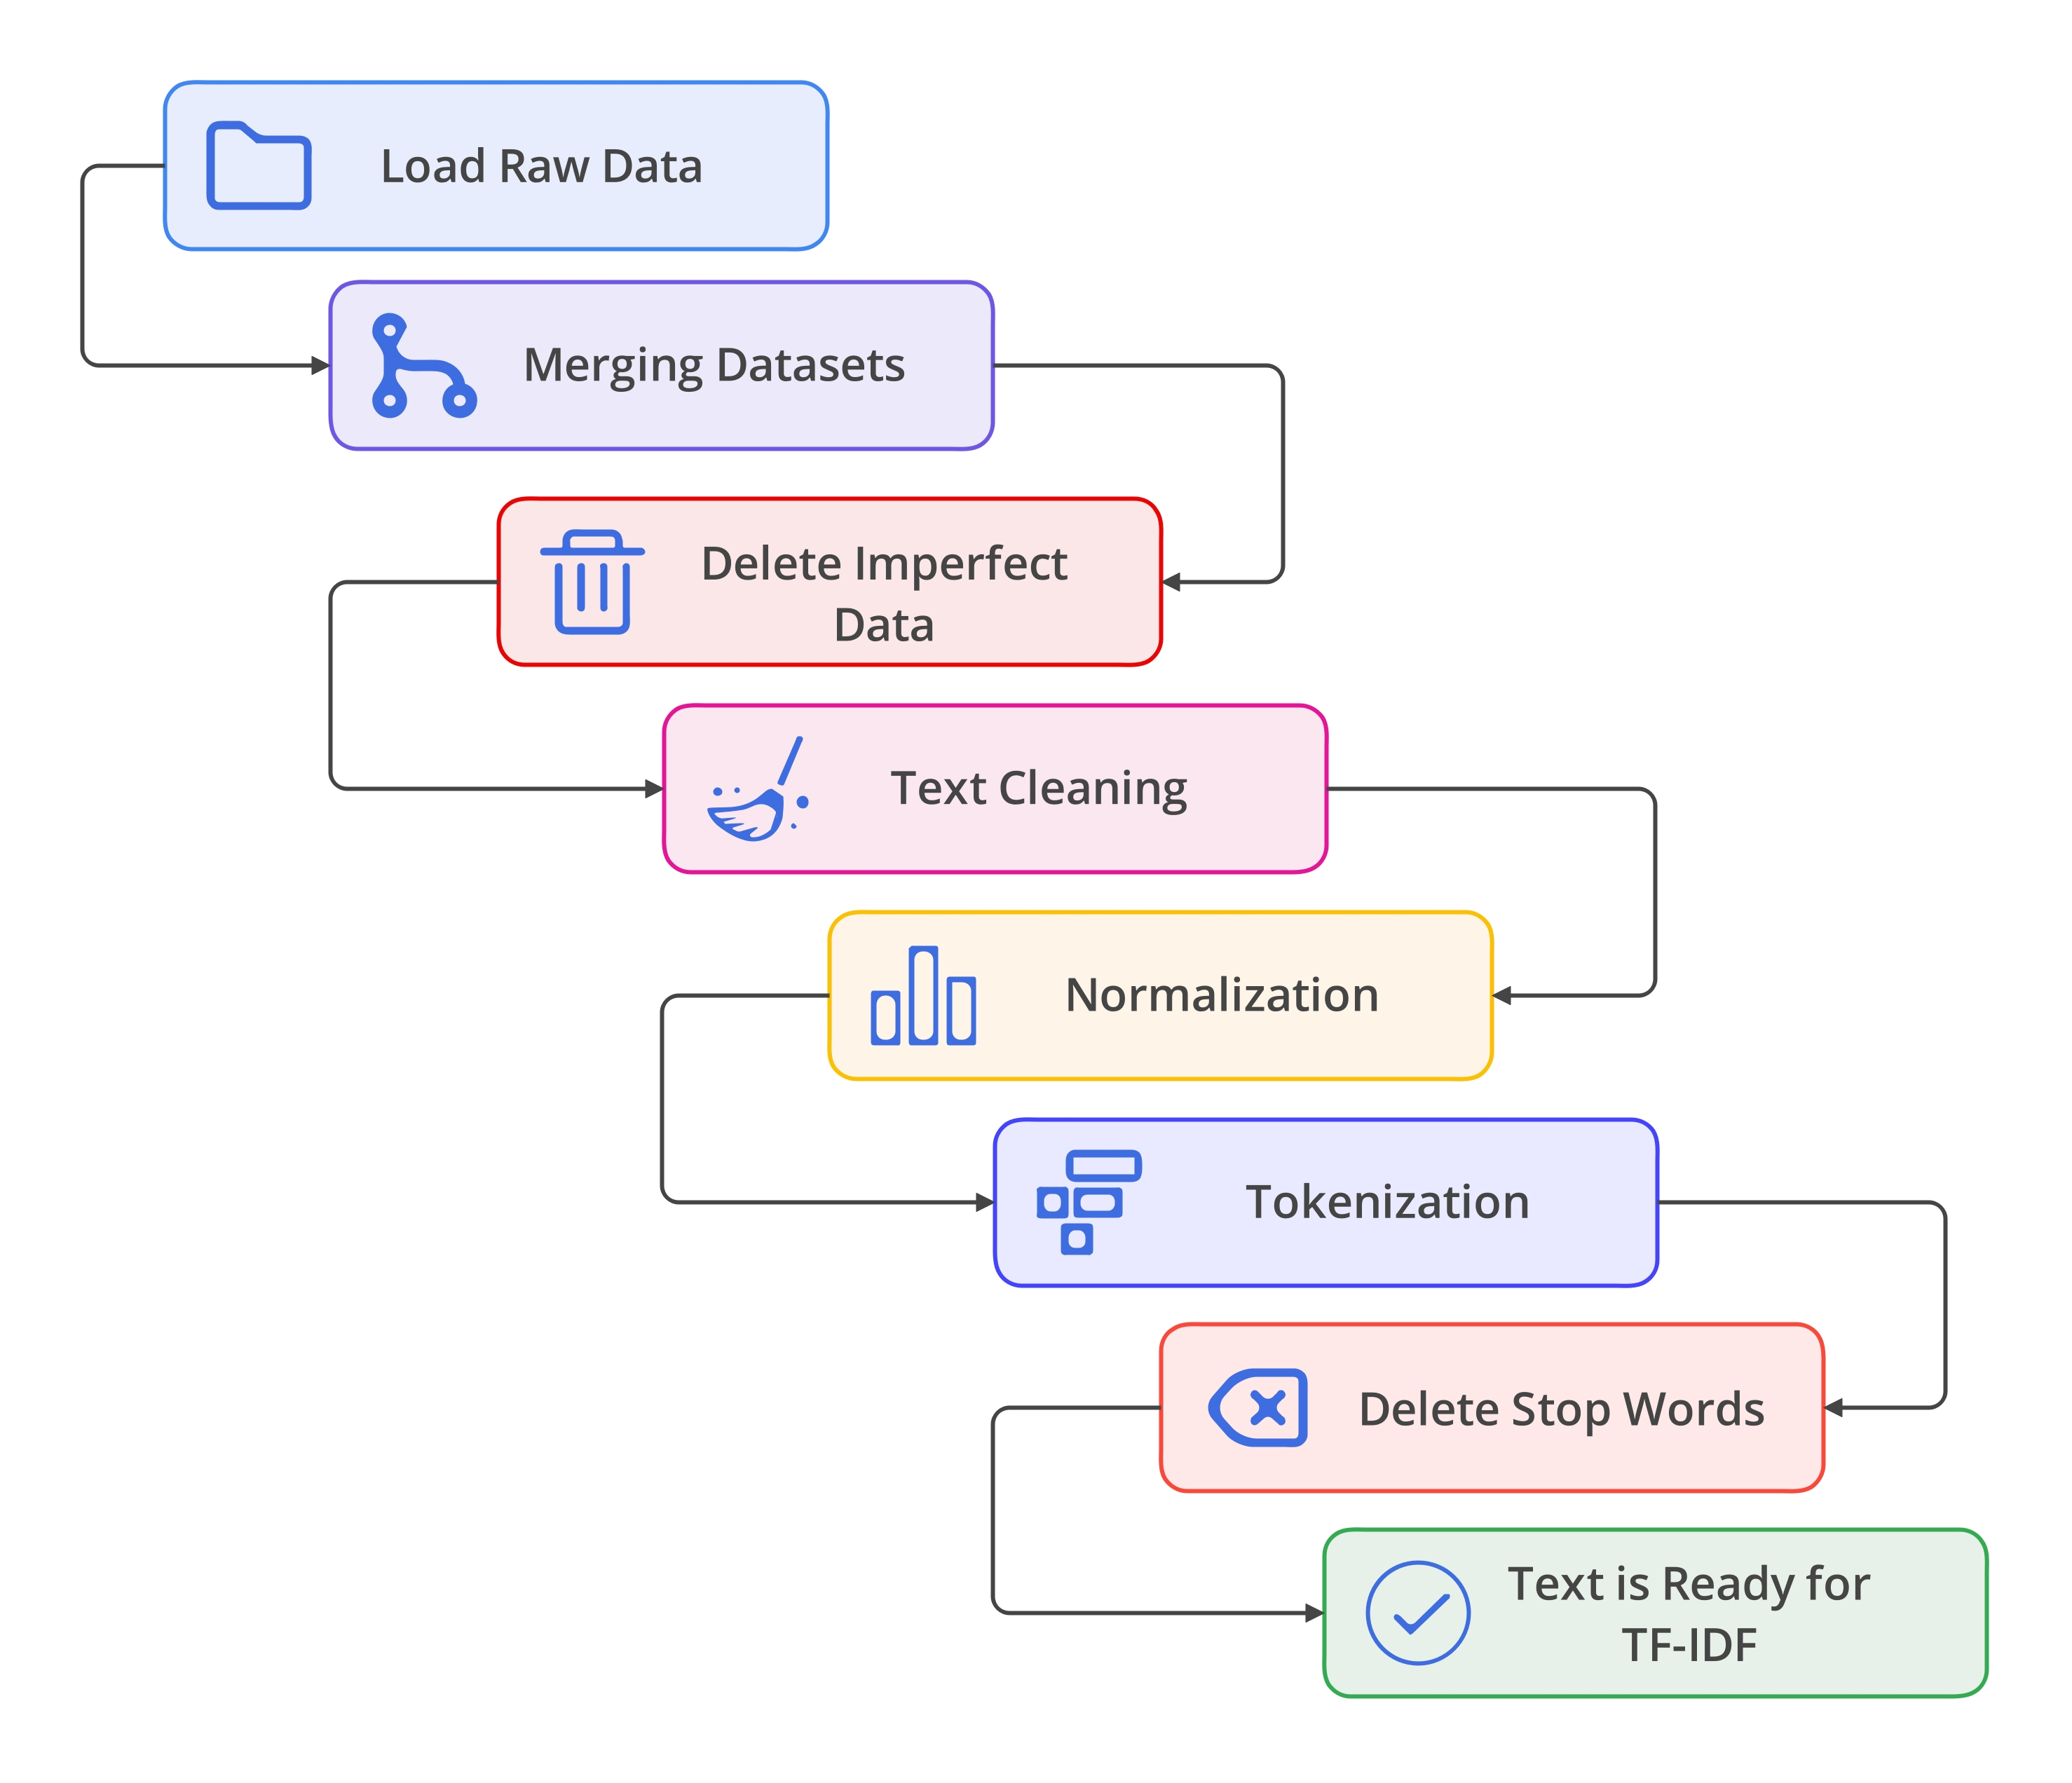
\includegraphics[width=1\textwidth]{figures/Drawing1.jpg}
 	\caption{فرآیند آماده‌سازی داده‌های متنی پیش از آموزش مدل}
 	\label{fig:textpreparing}
 \end{figure}
 
 \section{استخراج ویژگی‌ها \lr{(Feature Engineering)}}
 پس از تکمیل مرحله پیش‌پردازش، داده‌های متنی و اطلاعات جانبی محصولات برای استفاده در الگوریتم‌های یادگیری ماشین به ویژگی‌های قابل پردازش تبدیل شدند. این مرحله که با عنوان استخراج ویژگی شناخته می‌شود، یکی از مهم‌ترین مراحل توسعه مدل‌های یادگیری ماشین است؛ زیرا کیفیت و نوع ویژگی‌های استخراج‌شده تأثیر مستقیمی بر دقت و عملکرد مدل نهایی دارند.
 
 در این پروژه، علاوه بر ویژگی‌های استخراج‌شده از متن نظرات، از اطلاعات موجود در مجموعه داده محصولات و نظرات نیز استفاده شد تا مدل بتواند با در نظر گرفتن عوامل مختلف، تصمیم دقیق‌تری در تشخیص احساسات کاربران اتخاذ کند. ویژگی‌های استخراج‌شده در هفت گروه اصلی طبقه‌بندی شده‌اند.
 \subsection{ویژگی‌های متنی \lr{(Text Features)}}
 ویژگی‌های متنی از خود متن نظرات استخراج شدند و اطلاعاتی درباره ساختار و اندازه متن در اختیار مدل قرار دادند. این ویژگی‌ها شامل تعداد کاراکترهای متن، تعداد کلمات، میانگین طول کلمات و سایر شاخص‌های آماری مرتبط با متن هستند. علاوه بر این، متن‌های پیش‌پردازش‌شده با استفاده از روش TF-IDF به بردارهای عددی تبدیل شدند تا الگوریتم‌های یادگیری ماشین بتوانند آن‌ها را پردازش کنند. این دسته از ویژگی‌ها مهم‌ترین منبع اطلاعات برای تشخیص احساس موجود در هر نظر محسوب می‌شوند.
 \subsection{ویژگی‌های امتیازدهی \lr{(Rating Features)}}
 امتیاز ثبت‌شده توسط کاربران یکی از مهم‌ترین شاخص‌های تعیین احساس است. در این پروژه، علاوه بر استفاده از امتیاز هر نظر، اختلاف امتیاز ثبت‌شده با میانگین امتیاز همان محصول نیز به‌عنوان یک ویژگی استخراج شد. این ویژگی می‌تواند رفتار غیرمعمول کاربران و میزان اختلاف نظر آن‌ها با سایر خریداران را مشخص کرده و در بهبود عملکرد مدل مؤثر باشد.
 \subsection{ویژگی‌های پیشنهاد خرید \lr{(Recommendation Features)}}
 در دیجی‌کالا کاربران می‌توانند پس از ثبت نظر، محصول را به سایر افراد پیشنهاد دهند یا عدم پیشنهاد خود را اعلام کنند. این اطلاعات به‌صورت ویژگی دودویی \lr{(Binary Feature)} به مدل اضافه شدند. وجود این ویژگی ارتباط مستقیمی با احساس کاربران نسبت به محصول داشته و یکی از عوامل مؤثر در افزایش دقت مدل محسوب می‌شود.
 \subsection{ویژگی‌های وضعیت خریدار \lr{(Buyer Features)}}
 در مجموعه داده، مشخص شده است که آیا ثبت‌کننده نظر، خریدار واقعی محصول بوده است یا خیر. نظرات ثبت‌شده توسط خریداران واقعی معمولاً اعتبار بیشتری دارند و بیانگر تجربه عملی استفاده از محصول هستند. بنابراین این ویژگی نیز به‌صورت یک متغیر دودویی در فرآیند آموزش مدل مورد استفاده قرار گرفت.
 \subsection{ویژگی‌های قیمت \lr{(Price Features)}}
اطلاعات مربوط به قیمت محصولات نیز در فرآیند استخراج ویژگی مورد استفاده قرار گرفت. ویژگی‌هایی مانند قیمت نهایی محصول، میزان تخفیف و وضعیت موجودی کالا استخراج شدند. این اطلاعات می‌توانند در تحلیل رفتار کاربران مؤثر باشند؛ زیرا میزان رضایت مشتریان در بسیاری از موارد تحت تأثیر قیمت و ارزش خرید محصول قرار دارد.
\subsection{ویژگی‌های واکنش کاربران \lr{(Reaction Features)}}
هر نظر در دیجی‌کالا می‌تواند توسط سایر کاربران لایک یا دیسلایک شود. در این پروژه تعداد لایک‌ها، تعداد دیسلایک‌ها و نسبت لایک به کل واکنش‌ها به‌عنوان ویژگی‌های مستقل استخراج شدند. این ویژگی‌ها میزان تأیید یا مخالفت سایر کاربران با هر نظر را نشان داده و می‌توانند به تشخیص اعتبار و جهت‌گیری احساس موجود در آن کمک کنند.
\subsection{ویژگی‌های زمانی \lr{(Temporal Features)}}
زمان ثبت هر نظر نیز به‌عنوان یکی از منابع اطلاعاتی مورد استفاده قرار گرفت. با استخراج اطلاعاتی مانند روز، ماه و فصل از تاریخ ثبت نظرات (بر اساس تقویم جلالی)، ویژگی‌های زمانی ایجاد شدند. این ویژگی‌ها امکان بررسی تغییرات احساس کاربران در بازه‌های زمانی مختلف و تحلیل الگوهای رفتاری را فراهم می‌کنند.

در پایان این مرحله، تمامی ویژگی‌های استخراج‌شده در کنار بردارهای متنی حاصل از TF-IDF به‌عنوان ورودی مدل‌های یادگیری ماشین مورد استفاده قرار گرفتند. ترکیب ویژگی‌های متنی با اطلاعات جانبی محصولات و کاربران باعث شد مدل علاوه بر محتوای متن، عوامل مؤثر دیگر را نیز در فرآیند تصمیم‌گیری در نظر بگیرد و در نتیجه عملکرد دقیق‌تر و قابل‌اعتمادتری ارائه دهد.
\begin{table}[H]
	\centering
	\caption{دسته‌بندی ویژگی‌های استخراج‌شده}
	\label{tab:feature_groups}
	
	\begin{tabular}{p{4cm} p{9cm}}
		\toprule
		\textbf{گروه ویژگی} & \textbf{نمونه ویژگی‌ها} \\
		\midrule
		
		ویژگی‌های متنی &
		تعداد کلمات، تعداد کاراکترها، TF-IDF \\
		
		ویژگی‌های امتیاز &
		Rating، اختلاف با میانگین امتیاز محصول \\
		
		پیشنهاد خرید &
		پیشنهاد می‌کنم، پیشنهاد نمی‌کنم \\
		
		وضعیت خریدار &
		خریدار واقعی یا کاربر عادی \\
		
		ویژگی‌های قیمت &
		قیمت محصول، درصد تخفیف، وضعیت موجودی \\
		
		واکنش کاربران &
		تعداد لایک، تعداد دیسلایک، نسبت لایک به دیسلایک \\
		
		ویژگی‌های زمانی &
		روز ثبت نظر، ماه، فصل \\
		
		\bottomrule
	\end{tabular}
\end{table}
\section{آموزش مدل‌های یادگیری ماشین}
پس از تکمیل مراحل پیش‌پردازش و استخراج ویژگی‌ها، داده‌های آماده‌شده برای آموزش مدل‌های یادگیری ماشین مورد استفاده قرار گرفتند. هدف این مرحله، بررسی عملکرد الگوریتم‌های مختلف در طبقه‌بندی احساسات نظرات کاربران و انتخاب مناسب‌ترین مدل برای استفاده در سامانه نهایی بود. با توجه به ماهیت داده‌ها که شامل متون فارسی تبدیل‌شده به بردارهای TF-IDF با ابعاد بالا هستند، سه الگوریتم پرکاربرد و شناخته‌شده در حوزه طبقه‌بندی متن انتخاب شدند. عملکرد هر مدل بر اساس معیارهایی مانند دقت (Accuracy) ، دقت کلاس‌ها (Precision) ، بازخوانی (Recall) و امتیاز F1 مورد ارزیابی و مقایسه قرار گرفت.
\subsection{مدل \lr{Logistic Regression}}
 یکی از ساده‌ترین و در عین حال مؤثرترین الگوریتم‌های طبقه‌بندی است که در بسیاری از مسائل پردازش متن عملکرد قابل قبولی ارائه می‌دهد. این مدل با استفاده از یک تابع لجستیک، احتمال تعلق هر نمونه به کلاس‌های مختلف را محاسبه کرده و بر اساس بیشترین احتمال، کلاس نهایی را تعیین می‌کند.

در این پروژه، از \lr{Logistic Regression} به‌عنوان یکی از مدل‌های پایه (Baseline) استفاده شد تا عملکرد آن با سایر الگوریتم‌ها مقایسه شود. این مدل به دلیل سرعت مناسب، سادگی پیاده‌سازی و عملکرد مطلوب روی داده‌های با ابعاد بالا، گزینه مناسبی برای تحلیل احساسات متنی محسوب می‌شود.

مزایا:
\begin{itemize}
	\item سرعت بالای آموزش و پیش‌بینی
	\item عملکرد مناسب روی داده‌های متنی مبتنی بر TF-IDF
	\item سادگی پیاده‌سازی و تفسیر نتایج
	\item مصرف نسبتاً کم منابع پردازشی
\end{itemize}
معایب:
\begin{itemize}
	\item توانایی محدود در مدل‌سازی روابط پیچیده بین ویژگی‌ها
	\item حساسیت به تنظیم پارامترها و توزیع داده‌ها
	\item کاهش عملکرد در داده‌های بسیار نامتوازن
\end{itemize}



\subsection{مدل \lr{Linear Support Vector Machine (Linear SVM)}}
الگوریتم \lr{Linear Support Vector Machine (LinearSVC)} یکی از موفق‌ترین روش‌های طبقه‌بندی متن در حوزه پردازش زبان طبیعی است. این الگوریتم تلاش می‌کند با یافتن بهترین ابرصفحه \lr{(Hyperplane)} ، بیشترین فاصله ممکن را میان کلاس‌های مختلف ایجاد کرده و مرز تصمیم‌گیری مناسبی برای طبقه‌بندی داده‌ها به دست آورد.

دلیل اصلی انتخاب این مدل، عملکرد بسیار مناسب آن روی داده‌های متنی با ابعاد بالا و بردارهای TF-IDF است. در بسیاری از مسائل طبقه‌بندی متن، LinearSVM نسبت به سایر الگوریتم‌های کلاسیک دقت بیشتری ارائه می‌دهد و به همین دلیل یکی از گزینه‌های اصلی این پروژه محسوب می‌شد.

مزایا:
\begin{itemize}
	\item دقت بالا در طبقه‌بندی داده‌های متنی
	\item عملکرد مناسب در داده‌های با تعداد ویژگی زیاد
	\item مقاومت مناسب در برابر بیش‌برازش \lr{(Overfitting)}
	\item سرعت مناسب در فرآیند پیش‌بینی
\end{itemize}
معایب:
\begin{itemize}
	\item نیاز به تنظیم مناسب ابرپارامترها
	\item عدم ارائه احتمال کلاس‌ها به‌صورت مستقیم
	\item کاهش کارایی در مسائل غیرخطی بدون استفاده از Kernel
\end{itemize}
نتایج ارزیابی نشان داد که این مدل بهترین عملکرد را در میان مدل‌های بررسی‌شده داشته و پس از بهینه‌سازی نیز به‌عنوان مدل نهایی سامانه انتخاب شد.
\subsection{مدل \lr{Random Forest}}
 یک الگوریتم مبتنی بر مجموعه‌ای از درخت‌های تصمیم \lr{(Decision Trees)} است که با ترکیب نتایج چندین درخت، تصمیم نهایی را اتخاذ می‌کند. این روش معمولاً در مسائل طبقه‌بندی و رگرسیون عملکرد قابل قبولی داشته و نسبت به یک درخت تصمیم منفرد، پایداری بیشتری دارد.

در این پروژه، \lr{Random Forest} به‌عنوان یکی از مدل‌های مقایسه‌ای مورد استفاده قرار گرفت تا عملکرد آن در کنار سایر الگوریتم‌ها بررسی شود. اگرچه این مدل در بسیاری از مسائل ساختاریافته نتایج بسیار خوبی ارائه می‌دهد، اما در داده‌های متنی با تعداد ویژگی بسیار زیاد، معمولاً نسبت به الگوریتم‌هایی مانند LinearSVM عملکرد ضعیف‌تری دارد.

مزایا:
\begin{itemize}
	\item مقاومت مناسب در برابر بیش‌برازش
	\item توانایی مدل‌سازی روابط غیرخطی
	\item عدم حساسیت زیاد به داده‌های نویزی
	\item قابلیت بررسی اهمیت ویژگی‌ها \lr{(Feature Importance)}
\end{itemize}
معایب:
\begin{itemize}
	\item مصرف حافظه و زمان آموزش بیشتر نسبت به مدل‌های خطی
	\item کاهش کارایی در داده‌های متنی با ابعاد بسیار بالا
	\item پیچیدگی بیشتر در مقایسه با مدل‌های خطی
\end{itemize}
\subsection{مقایسه اولیه مدل‌ها}
پس از آموزش هر سه الگوریتم، عملکرد آن‌ها روی دیتاست آزمون مورد ارزیابی قرار گرفت. نتایج نشان داد که هر سه مدل عملکرد قابل قبولی در طبقه‌بندی احساسات داشتند، اما مدل LinearSVM توانست بهترین توازن را میان دقت، سرعت و توانایی تعمیم به داده‌های جدید ارائه دهد. به همین دلیل، این مدل برای مرحله بهینه‌سازی انتخاب شد تا با استفاده از تکنیک‌هایی مانند تنظیم ابرپارامترها و بهبود ویژگی‌ها، عملکرد آن بیش از پیش افزایش یابد.

جدول مقایسه نتایج اولیه مدل‌ها در فصل بعد ارائه شده و فرآیند بهینه‌سازی مدل منتخب به‌صورت کامل مورد بررسی قرار خواهد گرفت.
\begin{table}[H]
	\centering
	\caption{مقایسه دقت مدل‌های یادگیری ماشین}
	\label{tab:model_accuracy}
	
	\begin{latin}
		\begin{tabular}{lc}
			\toprule
			\textbf{Model} & \textbf{Accuracy} \\
			\midrule
			
			Logistic Regression & 65.2\% \\
			Linear SVM & \textbf{72.3\%} \\
			Random Forest & 68.6\% \\
			
			\bottomrule
		\end{tabular}
	\end{latin}
	
\end{table}

\begin{figure}[H]
	\centering
	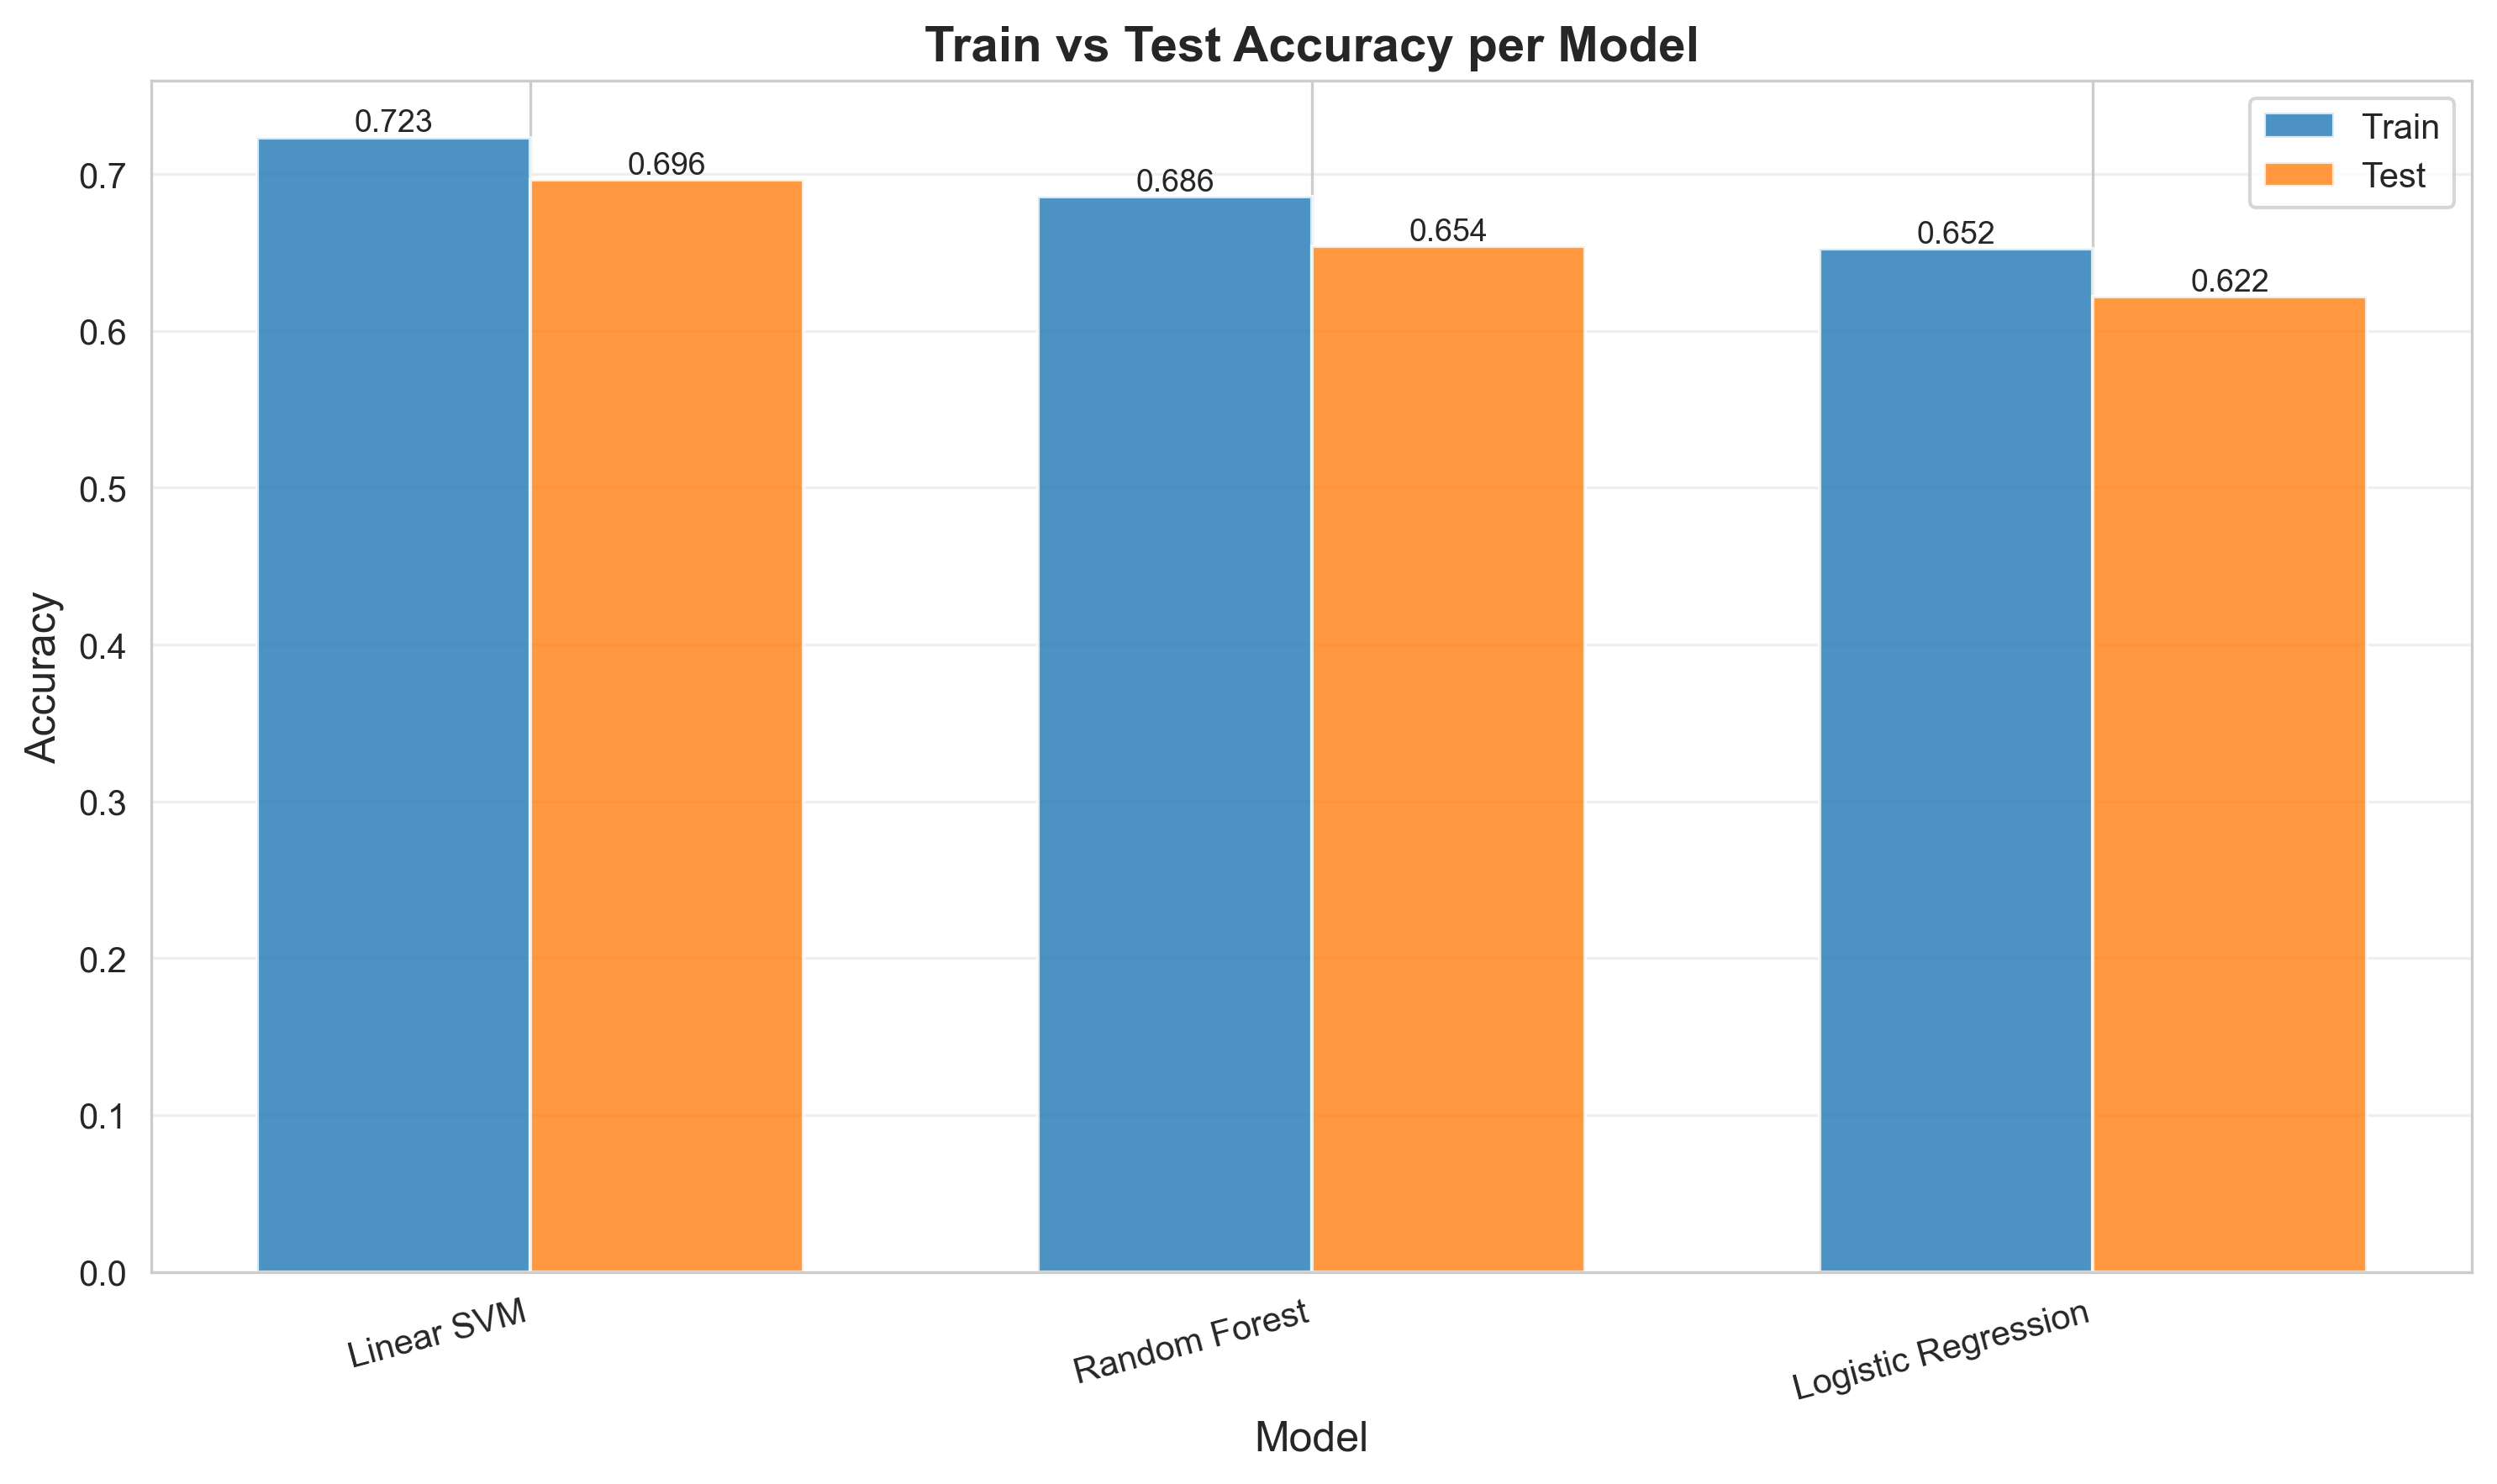
\includegraphics[width=1\textwidth]{figures/model_comparison.png}
	\caption{مقایسه دقت مدل‌ها یادگیری ماشین در تست و یادگیری}
	\label{fig:modelcompare}
\end{figure}

\textit{بر اساس نتایج اولیه، مدل LinearSVM بهترین عملکرد را در بین مدل‌های مورد بررسی داشت و برای مرحله بهینه‌سازی انتخاب شد.}

\section{بهبود مدل \lr{(Model Improvement)}}
پس از ارزیابی اولیه مدل‌های یادگیری ماشین، مشخص شد که اگرچه نتایج به‌دست‌آمده قابل قبول هستند، اما هنوز امکان افزایش دقت و بهبود توانایی مدل در تشخیص احساسات وجود دارد. به همین دلیل، مجموعه‌ای از روش‌های بهینه‌سازی بر روی مدل‌ها اعمال شد تا علاوه بر افزایش دقت، تعادل بهتری میان کلاس‌های مختلف برقرار شود. در این مرحله، از روش‌هایی مانند بهینه‌سازی بردارسازی متن، تنظیم ابرپارامترها، متعادل‌سازی داده‌ها و ترکیب مدل‌ها استفاده شد.
\subsection{بهینه‌سازی ویژگی‌های متنی با TF-IDF}
یکی از عوامل مؤثر در عملکرد مدل‌های طبقه‌بندی متن، نحوه نمایش داده‌های متنی به‌صورت بردارهای عددی است. در این پروژه، از روش TF-IDF \lr{(Term Frequency-Inverse Document Frequency)} برای تبدیل متن به بردارهای عددی استفاده شد. این روش با در نظر گرفتن میزان تکرار هر واژه در یک متن و میزان اهمیت آن در کل مجموعه داده، وزن مناسبی به کلمات اختصاص می‌دهد.

برای افزایش کیفیت ویژگی‌های استخراج‌شده، پارامترهای TF-IDF مورد بررسی و بهینه‌سازی قرار گرفتند. مهم‌ترین تنظیمات اعمال‌شده عبارت بودند از:

\begin{itemize}
	\item استفاده از Unigram ، Bigram و \lr{Trigram (ngram range=(1,3))}
	\item محدود کردن تعداد ویژگی‌ها به 8000 ویژگی
	\item حذف کلمات بسیار نادر و بسیار پرتکرار
	\item استفاده از \lr{Sublinear TF} برای کاهش تأثیر کلمات با فراوانی بسیار زیاد
\end{itemize}
 




این تنظیمات باعث شدند نمایش عددی متن‌ها اطلاعات بیشتری از ساختار جملات و ترکیب واژه‌ها را در اختیار مدل قرار دهد.
\subsection{تنظیم ابرپارامترها با GridSearchCV}
هر الگوریتم یادگیری ماشین دارای مجموعه‌ای از پارامترهای قابل تنظیم است که انتخاب مناسب آن‌ها تأثیر مستقیمی بر عملکرد مدل دارد. برای یافتن بهترین ترکیب این پارامترها، از روش GridSearchCV استفاده شد.

در این روش، ترکیب‌های مختلفی از مقادیر پارامترها به‌صورت خودکار آزمایش شده و عملکرد هر ترکیب با استفاده از اعتبارسنجی متقابل \lr{(Cross Validation) } ارزیابی گردید. برای مدل LinearSVC  پارامترهایی مانند مقدار C و \lr{Class Weight} بررسی شدند و در نهایت ترکیب زیر بهترین نتیجه را ارائه داد:
\begin{latin}
	\begin{lstlisting}[language=Python]
		C = 0.1
		Class Weight = Balanced
	\end{lstlisting}
\end{latin}

استفاده از این مقادیر باعث افزایش توانایی مدل در تفکیک کلاس‌های مختلف، به‌ویژه کلاس‌های کم‌تعداد، شد.
\subsection{متعادل‌سازی داده‌ها با SMOTE}
یکی از چالش‌های این پروژه، نامتوازن بودن توزیع کلاس‌ها بود؛ به‌طوری‌که تعداد نظرات مثبت به‌مراتب بیشتر از نظرات منفی و خنثی بود. این موضوع می‌تواند باعث شود مدل تمایل بیشتری به پیش‌بینی کلاس غالب داشته باشد.

برای کاهش این مشکل، از الگوریتم \lr{SMOTE (Synthetic Minority Oversampling Technique)} استفاده شد. این روش با تولید نمونه‌های مصنوعی برای کلاس‌های کم‌تعداد، تلاش می‌کند تعادل بهتری میان کلاس‌ها ایجاد کند.

اگرچه استفاده از SMOTE موجب متوازن‌تر شدن داده‌ها شد، اما در آزمایش‌های انجام‌شده، دقت نهایی مدل نسبت به نسخه بهینه‌شده بدون SMOTE کاهش یافت. بنابراین، این روش به‌عنوان مدل نهایی انتخاب نشد.
\subsection{استفاده از \lr{Voting Ensemble}}
به‌منظور بررسی امکان افزایش عملکرد سیستم، از روش \lr{Voting Ensemble} نیز استفاده شد. در این روش، خروجی سه مدل \lr{Logistic Regression} ، \lr{Random Forest} و LinearSVM با یکدیگر ترکیب شد و تصمیم نهایی بر اساس رأی‌گیری بین مدل‌ها اتخاذ گردید.

هدف از این روش، بهره‌گیری از نقاط قوت هر مدل و کاهش خطاهای احتمالی بود. هرچند مدل Ensemble نسبت به برخی مدل‌های منفرد عملکرد بهتری داشت، اما همچنان نتوانست از مدل بهینه‌شده LinearSVC پیشی بگیرد.
\subsection{انتخاب مدل نهایی}
پس از انجام تمامی مراحل بهینه‌سازی، عملکرد روش‌های مختلف با یکدیگر مقایسه شد. نتایج نشان داد که مدل LinearSVC پس از تنظیم ابرپارامترها و بهینه‌سازی TF-IDF ، بهترین عملکرد را در میان تمامی روش‌های بررسی‌شده ارائه می‌دهد.

این مدل توانست به دقت حدود 79٫45 درصد و مقدار \lr{Macro F1} برابر با 0٫634 دست یابد که نسبت به نسخه اولیه و سایر روش‌های آزمایش‌شده بهبود محسوسی را نشان می‌دهد. علاوه بر دقت بالاتر، سرعت مناسب در آموزش و پیش‌بینی، مصرف کمتر منابع پردازشی و عملکرد مطلوب در داده‌های متنی با ابعاد بالا از دیگر دلایل انتخاب این مدل به‌عنوان مدل نهایی سامانه بودند.

بر همین اساس، مدل بهینه‌شده LinearSVC ذخیره شده و در بخش Backend برای انجام پیش‌بینی احساسات کاربران مورد استفاده قرار گرفت.

\begin{table}[H]
	\centering
	\caption{مقایسه روش‌های بهبود مدل}
	\label{tab:model_improvement}
	
	\begin{latin}
		\begin{tabular}{lcc}
			\toprule
			\textbf{Method} & \textbf{Accuracy} & \textbf{Macro F1} \\
			\midrule
			
			Baseline & 76.09\% & 0.606 \\
			GridSearch + TF-IDF & \textbf{79.45\%} & \textbf{0.634} \\
			SMOTE & 73.77\% & 0.601 \\
			Voting Ensemble & 78.71\% & 0.630 \\
			
			\bottomrule
		\end{tabular}
	\end{latin}
\end{table}

\begin{figure}[H]
	\centering
	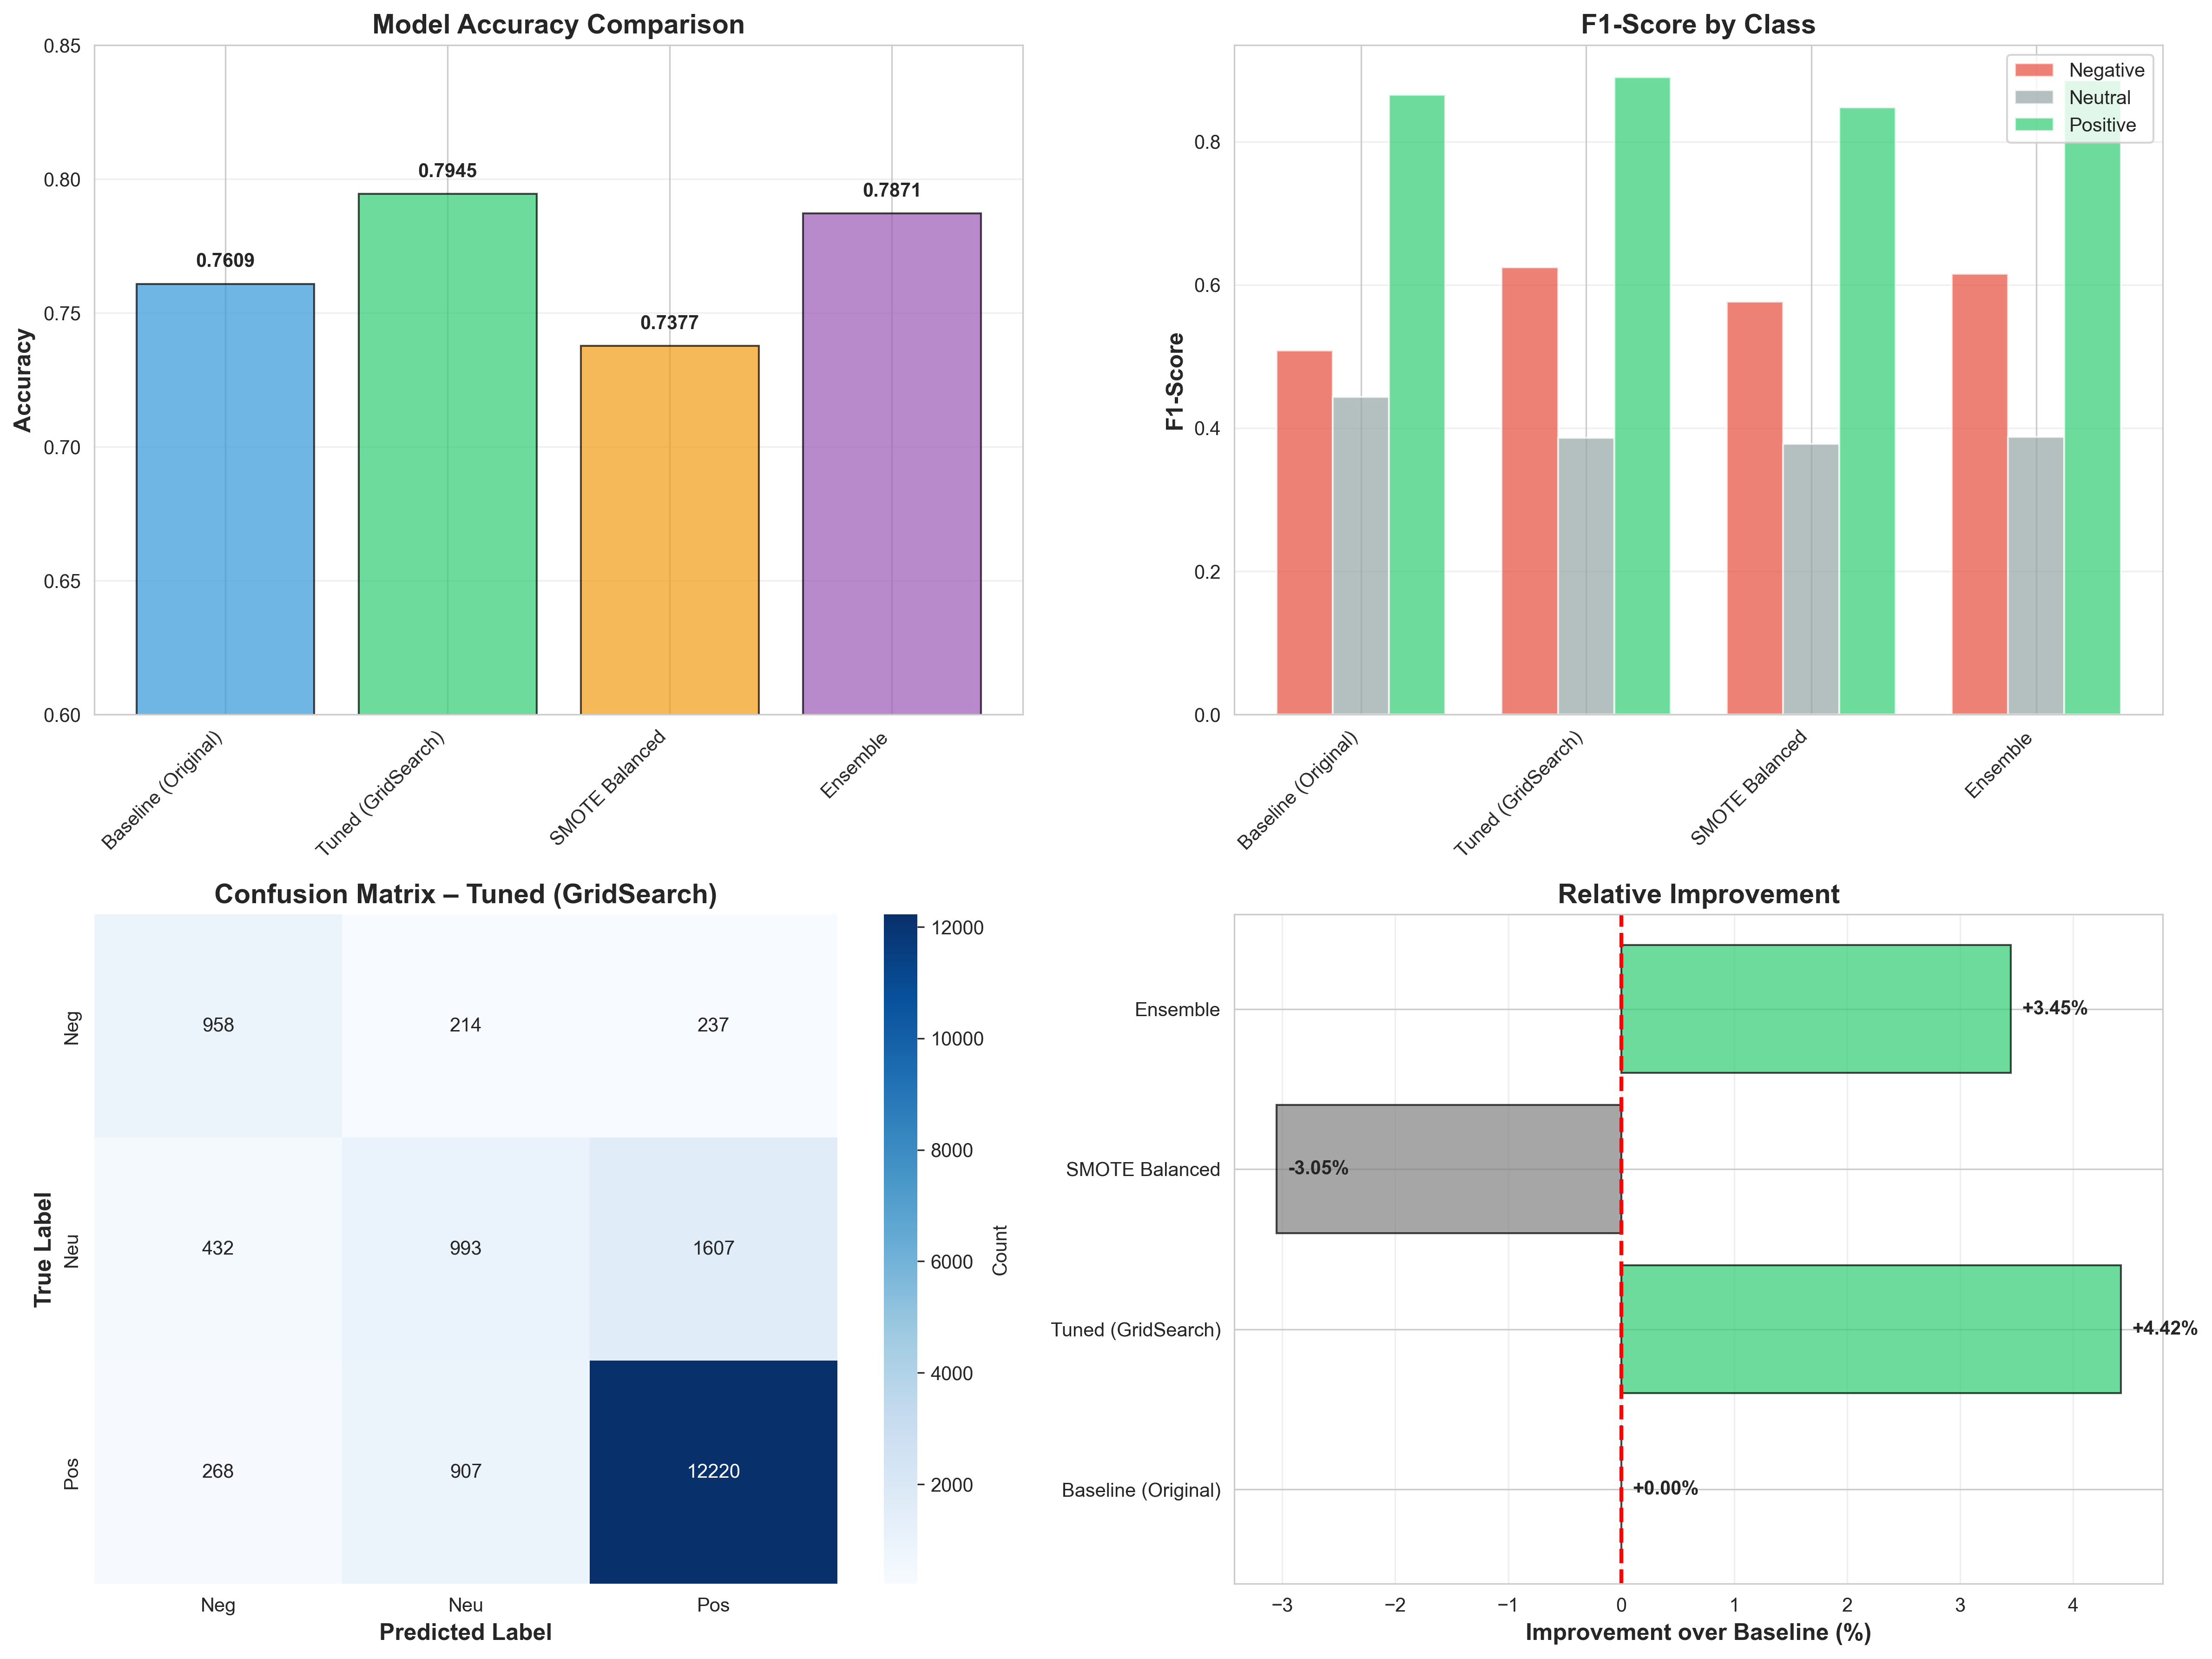
\includegraphics[width=1\textwidth]{figures/model_improvement_comparison.png}
	\caption{آمار کلی روش‌های بهبود مدل}
	\label{fig:modelimprovecompare}
\end{figure}
\section{نتایج و ارزیابی مدل}
پس از آموزش مدل‌های یادگیری ماشین و اعمال روش‌های مختلف بهینه‌سازی، عملکرد آن‌ها بر روی دیتاست تست مورد ارزیابی قرار گرفت. برای سنجش کیفیت مدل‌ها، از معیارهای متداول ارزیابی در مسائل طبقه‌بندی شامل Accuracy ، Precision ، Recall و \lr{Macro F1-Score } استفاده شد. همچنین، به‌منظور تحلیل دقیق‌تر نحوه عملکرد مدل در تشخیص هر کلاس، ماتریس درهم‌ریختگی \lr{(Confusion Matrix)} نیز مورد بررسی قرار گرفت.
\subsection{نتایج دقت (Accuracy)}
جدول \ref{tab:model_improvement} عملکرد روش‌های مختلف را از نظر دقت (Accuracy) نشان می‌دهد. همان‌طور که مشاهده می‌شود، استفاده از روش‌های بهینه‌سازی موجب افزایش قابل توجه دقت مدل نسبت به نسخه اولیه شده است.

نتایج نشان می‌دهد که استفاده از GridSearchCV در کنار تنظیم پارامترهای TF-IDF بیشترین تأثیر را در افزایش دقت مدل داشته و توانسته است عملکرد سیستم را نسبت به مدل اولیه حدود ۳ درصد بهبود دهد.
\subsection{نتایج معیار F1-Score}
از آنجا که توزیع کلاس‌های احساسات کاملاً متوازن نیست، تنها استفاده از معیار Accuracy برای ارزیابی مدل کافی نیست. به همین دلیل، از معیار \lr{Macro F1-Score } نیز استفاده شد تا عملکرد مدل در تمامی کلاس‌ها به‌صورت یکسان مورد بررسی قرار گیرد.

\begin{table}[H]
	\centering
	\caption{مقایسه روش‌های مختلف بر اساس معیار Macro F1}
	\label{tab:macro_f1_comparison}
	
	\begin{latin}
		\begin{tabular}{lc}
			\toprule
			\textbf{Method} & \textbf{Macro F1} \\
			\midrule
			
			Baseline & 0.606 \\
			GridSearch + TF-IDF & \textbf{0.634} \\
			SMOTE & 0.601 \\
			Voting Ensemble & 0.630 \\
			
			\bottomrule
		\end{tabular}
	\end{latin}
	
\end{table}

همان‌طور که مشاهده می‌شود، مدل بهینه‌شده LinearSVC علاوه بر دستیابی به بیشترین Accuracy ، بالاترین مقدار \lr{Macro F1} را نیز کسب کرده است که نشان‌دهنده عملکرد مناسب‌تر آن در طبقه‌بندی هر سه کلاس احساسات است.
\subsection{ماتریس درهم‌ریختگی \lr{(Confusion Matrix)}}
برای تحلیل دقیق‌تر عملکرد مدل، از ماتریس درهم‌ریختگی \lr{(Confusion Matrix)} استفاده شد. این ماتریس تعداد پیش‌بینی‌های صحیح و نادرست مدل را برای هر کلاس نمایش می‌دهد و مشخص می‌کند که مدل در تشخیص کدام کلاس‌ها عملکرد بهتری داشته و در کدام بخش‌ها دچار خطا شده است.

\begin{figure}[H]
	\centering
	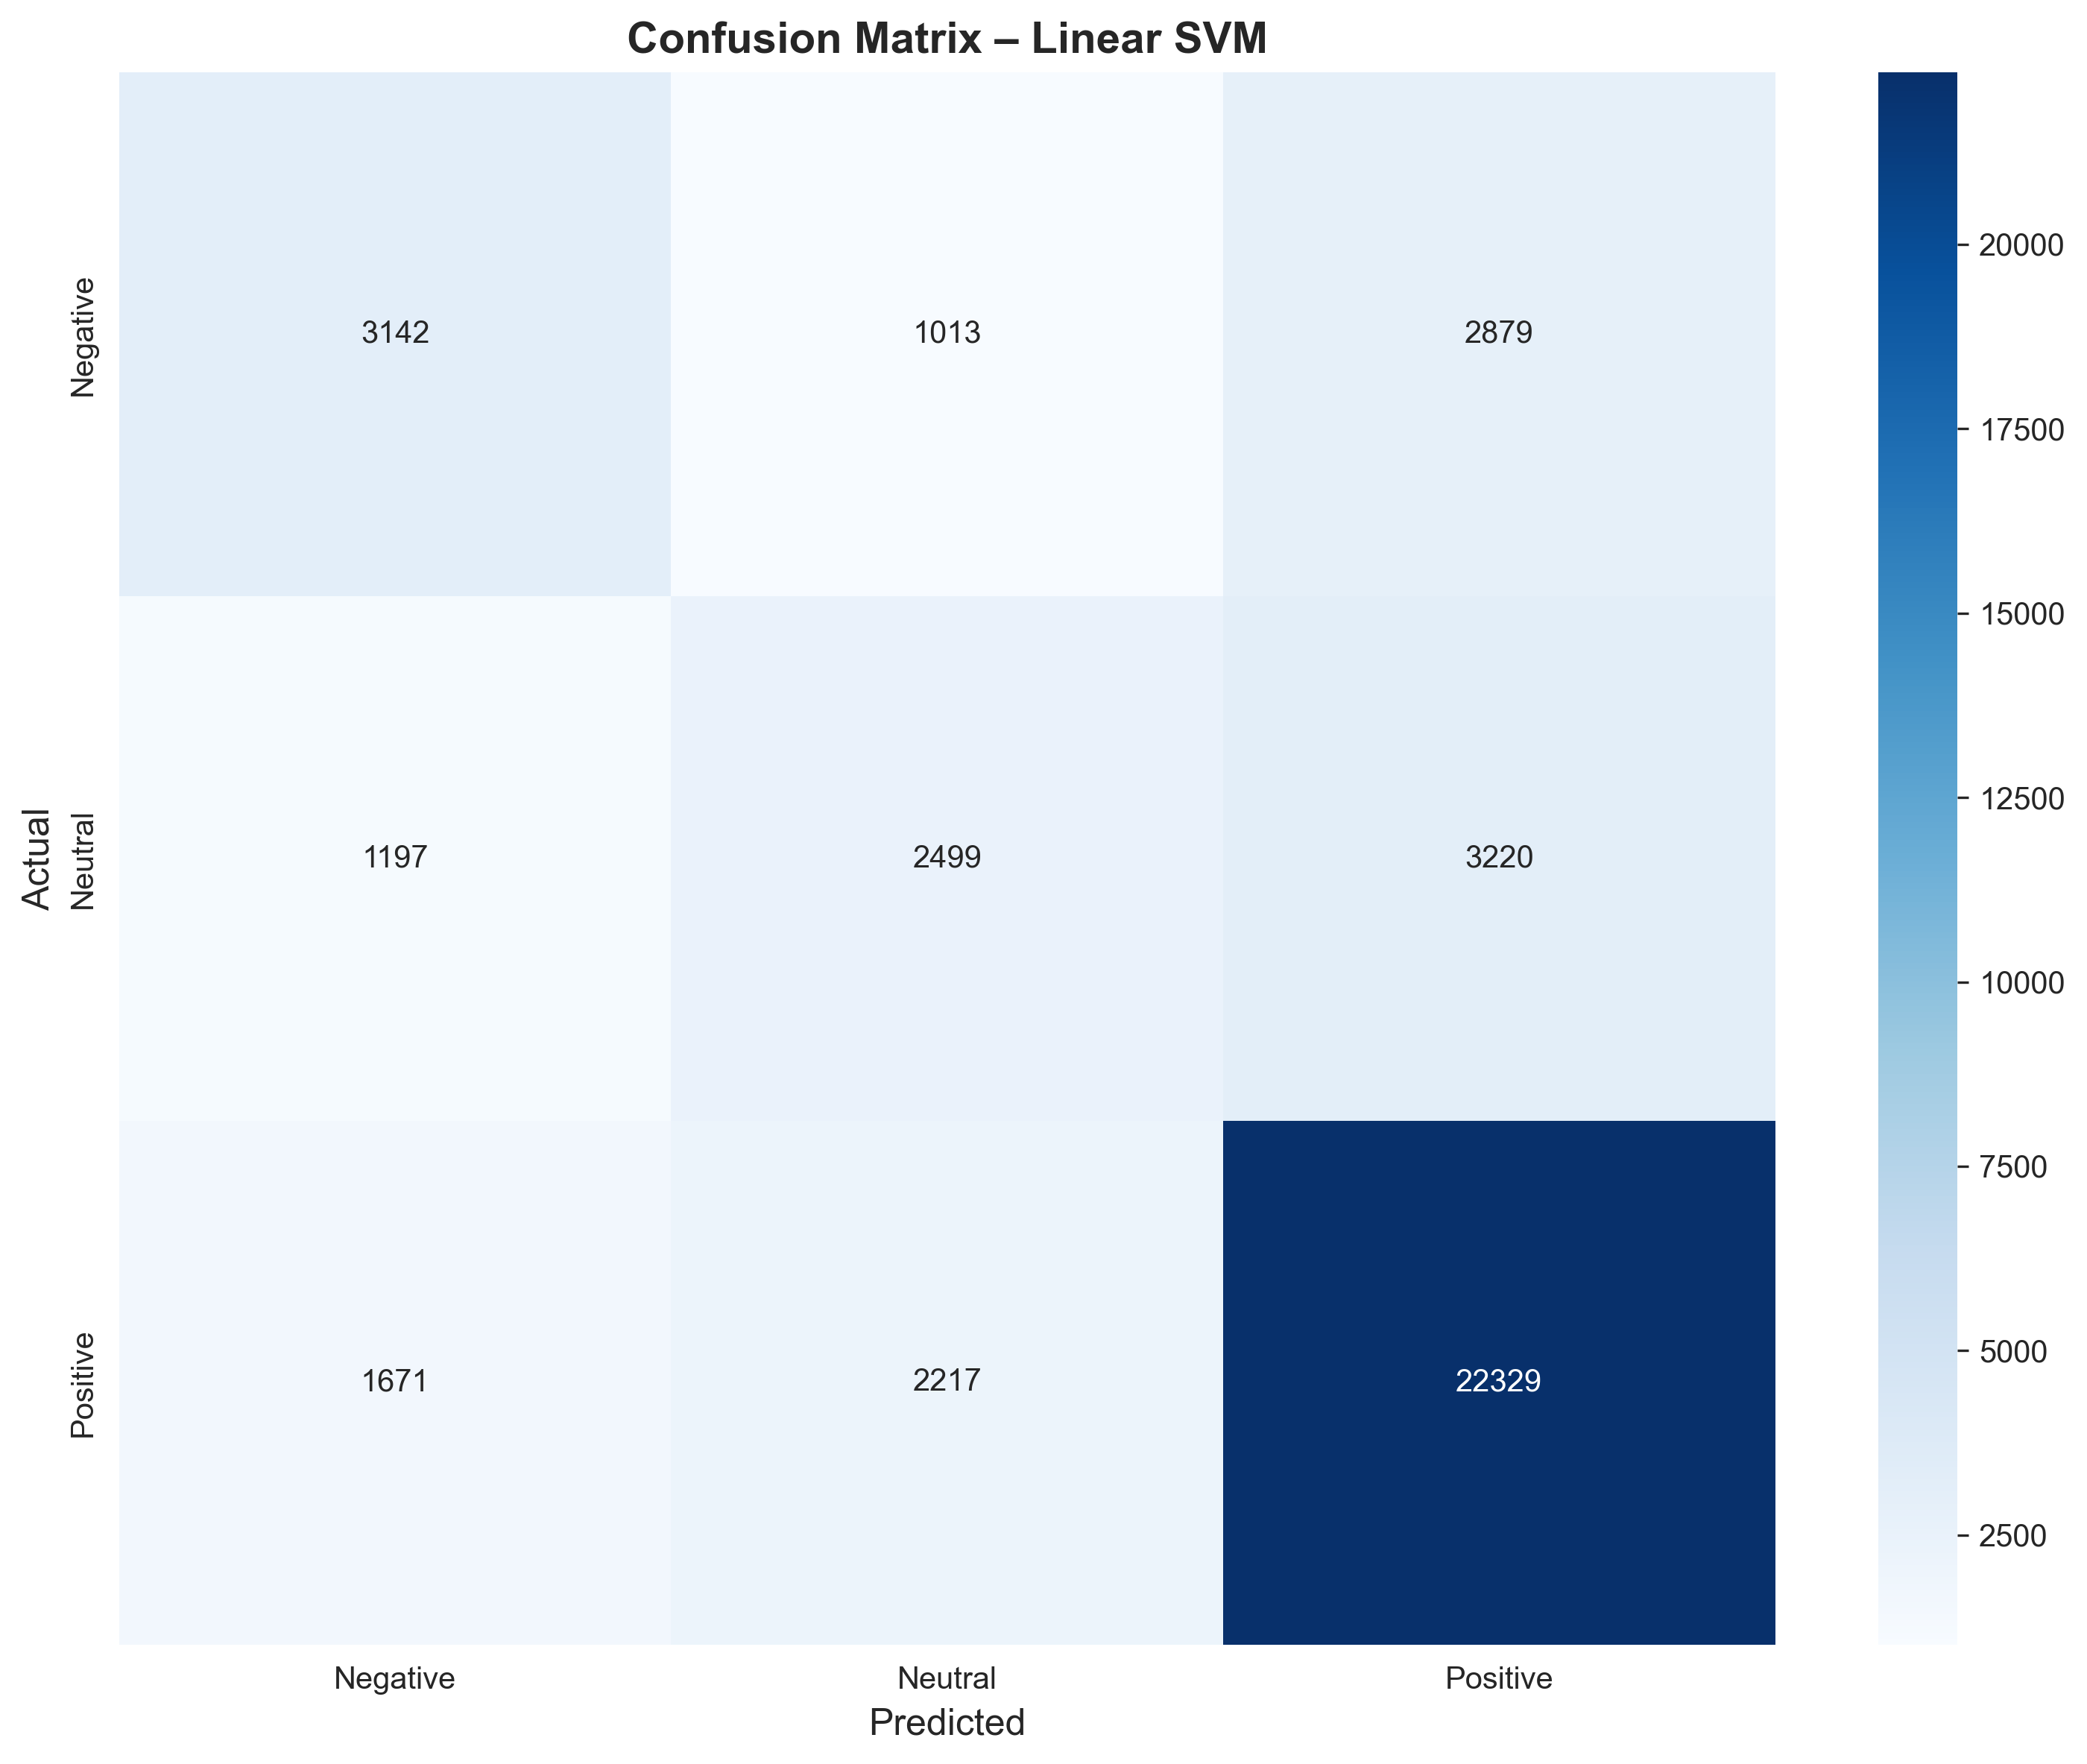
\includegraphics[width=1\textwidth]{figures/confusion_matrix_best_model.png}
	\caption{ماتریس درهم‌ریختگی مدل نهایی (LinearSVC)}
	\label{fig:confusionmatrix}
\end{figure}

بررسی ماتریس درهم‌ریختگی نشان می‌دهد که مدل در تشخیص نظرات مثبت عملکرد بسیار مطلوبی داشته و بیشتر نمونه‌های این کلاس را به‌درستی شناسایی کرده است. در مقابل، بیشترین میزان خطا مربوط به کلاس خنثی است؛ زیرا این دسته از نظرات معمولاً دارای ویژگی‌هایی مشترک با نظرات مثبت و منفی بوده و مرز مشخصی میان آن‌ها وجود ندارد. همچنین، بخش قابل توجهی از نمونه‌های کلاس منفی نیز به‌درستی شناسایی شده‌اند که نشان‌دهنده توانایی مناسب مدل در تشخیص احساسات منفی کاربران است.
\subsection{تحلیل نتایج}
نتایج به‌دست‌آمده نشان می‌دهد که استفاده از مراحل دقیق پیش‌پردازش، استخراج ویژگی‌های مناسب و بهینه‌سازی مدل تأثیر قابل توجهی بر افزایش عملکرد سیستم داشته است. مدل LinearSVC پس از تنظیم ابرپارامترها و بهینه‌سازی بردارسازی TF-IDF ، توانست بهترین نتایج را در میان تمامی روش‌های بررسی‌شده به دست آورد.

از سوی دیگر، آزمایش روش SMOTE نشان داد که اگرچه این تکنیک موجب متعادل‌تر شدن داده‌ها می‌شود، اما در این پروژه نتوانست عملکرد کلی مدل را بهبود دهد. همچنین، استفاده از \lr{Voting Ensemble} نسبت به مدل پایه نتایج بهتری ارائه کرد، اما همچنان اندکی ضعیف‌تر از مدل بهینه‌شده LinearSVC بود.

به‌طور کلی، نتایج ارزیابی نشان می‌دهد که مدل نهایی قادر است با دقت قابل قبول، احساس موجود در نظرات فارسی کاربران را تشخیص دهد و از این رو برای استفاده در سامانه تحلیل احساسات توسعه‌یافته مناسب است. با این حال، عملکرد پایین‌تر مدل در کلاس خنثی نشان می‌دهد که هنوز ظرفیت بهبود وجود دارد و استفاده از مدل‌های مبتنی بر یادگیری عمیق مانند ParsBERT می‌تواند در آینده موجب افزایش دقت و بهبود تشخیص این دسته از نظرات شود.
\section{طراحی و پیاده‌سازی Backend}
بخش Backend این پروژه با استفاده از فریم‌ورک FastAPI توسعه داده شده است و وظیفه مدیریت درخواست‌های کاربران، اجرای مدل یادگیری ماشین، برقراری ارتباط با پایگاه داده و ارائه اطلاعات موردنیاز به رابط کاربری را بر عهده دارد. طراحی این بخش به‌صورت ماژولار انجام شده است تا هر قسمت از سیستم مسئولیت مشخصی داشته باشد و توسعه یا نگهداری آن در آینده با سهولت بیشتری انجام شود.

معماری Backend به گونه‌ای طراحی شده است که پس از دریافت درخواست از کاربر، ابتدا داده‌های ورودی اعتبارسنجی شده، سپس عملیات پیش‌پردازش متن و پیش‌بینی احساس توسط مدل یادگیری ماشین انجام می‌شود. در ادامه، نتیجه در صورت نیاز در پایگاه داده ذخیره شده و پاسخ مناسب به کاربر بازگردانده می‌شود. این ساختار علاوه بر سادگی، امکان توسعه قابلیت‌های جدید بدون ایجاد تغییرات اساسی در سایر بخش‌های سیستم را فراهم می‌کند.
\subsection{استفاده از FastAPI}
برای توسعه API های پروژه از FastAPI استفاده شده است. FastAPI یکی از فریم‌ورک‌های مدرن زبان Python برای توسعه REST API محسوب می‌شود.

از دیگر مزایای FastAPI می‌توان به سادگی توسعه Endpoint های جدید، عملکرد مناسب در پردازش هم‌زمان درخواست‌ها و سازگاری کامل با کتابخانه‌های یادگیری ماشین اشاره کرد.
\subsection{ساختار Route ها}
به‌منظور افزایش خوانایی و قابلیت نگهداری پروژه، Endpoint های سیستم در قالب چند Route مستقل سازمان‌دهی شده‌اند که هرکدام مسئول بخشی از عملکرد سامانه هستند.
\begin{itemize}
	\item بخش تحلیل احساسات \lr{(Sentiment)}:
	این بخش وظیفه دریافت متن نظرات کاربران، اجرای مدل یادگیری ماشین و بازگرداندن نتیجه تحلیل احساسات را بر عهده دارد. علاوه بر پیش‌بینی یک نظر، امکان تحلیل هم‌زمان چندین نظر نیز در این قسمت پیاده‌سازی شده است.
	\item بخش تاریخچه \lr{(History)}:
	تمامی پیش‌بینی‌هایی که از طریق سرویس تحلیل تک‌نظر انجام می‌شوند، در پایگاه داده ذخیره می‌شوند. این بخش امکان مشاهده تاریخچه تحلیل‌ها، دریافت آمار کلی احساسات، مشاهده جزئیات هر رکورد و حذف اطلاعات ذخیره‌شده را فراهم می‌کند.
	\item بخش محصولات \lr{(Products)}:
	این Route اطلاعات مربوط به محصولات را در اختیار کاربران قرار می‌دهد. کاربران می‌توانند محصولات را جستجو کرده، اطلاعات مربوط به هر محصول را مشاهده کنند و علاوه بر آن، خلاصه‌ای از نظرات کاربران و توزیع احساسات ثبت‌شده برای آن محصول را دریافت نمایند.
\end{itemize}
\subsection{پایگاه داده}
برای ذخیره اطلاعات از پایگاه داده SQLite استفاده شده است. ارتباط برنامه با پایگاه داده نیز توسط \lr{SQLAlchemy ORM} و به‌صورت Asynchronous مدیریت می‌شود.

در این پروژه دو جدول اصلی در پایگاه داده وجود دارد:
\begin{enumerate}
	\item \lr{Prediction History}:
	 ذخیره متن ورودی کاربران، متن پیش‌پردازش‌شده، نتیجه تحلیل احساسات، میزان اطمینان مدل و زمان ثبت درخواست.
	 \item \lr{Product Summaries}:
	 ذخیره خلاصه تحلیل محصولات و نتایج محاسبه‌شده به‌منظور جلوگیری از پردازش مجدد در درخواست‌های بعدی.
\end{enumerate}
استفاده از مکانیزم Cache برای اطلاعات محصولات باعث کاهش زمان پاسخ‌گویی سیستم و جلوگیری از انجام محاسبات تکراری شده است.
\subsection{فرآیند پیش‌بینی احساسات \lr{(Prediction Flow)}}
فرآیند تحلیل احساسات در Backend شامل چند مرحله متوالی است. ابتدا متن ارسال‌شده توسط کاربر اعتبارسنجی شده و سپس همان مراحل پیش‌پردازش که در زمان آموزش مدل استفاده شده بودند، بر روی متن اعمال می‌شوند. در ادامه، متن پیش‌پردازش‌شده توسط بردارساز TF-IDF به نمایش عددی تبدیل شده و به مدل آموزش‌دیده LinearSVC ارسال می‌شود.

پس از انجام پیش‌بینی، برچسب احساس (مثبت، منفی یا خنثی) تعیین شده و با استفاده از مقدار \lr{Decision Function} مدل، یک مقدار Confidence نیز محاسبه می‌شود تا میزان اطمینان مدل نسبت به پیش‌بینی مشخص گردد. در نهایت، نتیجه برای کاربر ارسال شده و در صورت تحلیل تک‌نظر، اطلاعات در جدول تاریخچه نیز ذخیره می‌شود.
\subsection{مدیریت تاریخچه تحلیل‌ها}
هر بار که کاربر متنی را برای تحلیل ارسال می‌کند، اطلاعات مربوط به آن درخواست شامل متن اصلی، متن پیش‌پردازش‌شده، نتیجه تحلیل، میزان اطمینان مدل و زمان ثبت در پایگاه داده ذخیره می‌شود.

این قابلیت علاوه بر امکان مشاهده سوابق تحلیل، امکان تهیه آمار کلی از تعداد نظرات مثبت، منفی و خنثی و همچنین حذف یا بازیابی اطلاعات ذخیره‌شده را نیز فراهم می‌کند.
\subsection{خلاصه‌سازی نظرات محصولات \lr{(Product Summary)}}
یکی از قابلیت‌های کاربردی این پروژه، تولید خلاصه‌ای از مهم‌ترین نظرات کاربران درباره هر محصول است. هدف از این بخش، کاهش زمان موردنیاز برای مطالعه تعداد زیادی نظر و ارائه دیدگاهی کلی از نقاط قوت، نقاط ضعف و تجربه کاربران نسبت به یک محصول است.

در این پروژه، برای تولید خلاصه از مدل زبانی \lr{Qwen3 (Large Language Model)} استفاده شده است. پس از دریافت درخواست کاربر، تمامی نظرات مربوط به محصول موردنظر جمع‌آوری شده و پس از انجام مراحل لازم برای آماده‌سازی متن، به مدل Qwen3 ارسال می‌شوند. این مدل با درک معنایی نظرات، مهم‌ترین اطلاعات موجود در میان دیدگاه‌های کاربران را استخراج کرده و خلاصه‌ای روان، منسجم و قابل فهم تولید می‌کند.

استفاده از مدل Qwen3 این امکان را فراهم می‌کند که خلاصه تولیدشده صرفاً بر اساس فراوانی کلمات نباشد، بلکه مفهوم کلی نظرات نیز در نظر گرفته شود. در نتیجه، مدل می‌تواند نقاط قوت و ضعف تکرارشونده، موضوعات پرتکرار و دیدگاه کلی کاربران نسبت به محصول را به‌صورت یک متن طبیعی و خوانا ارائه دهد. این ویژگی باعث می‌شود کیفیت خلاصه‌های تولیدشده نسبت به روش‌های کلاسیک استخراجی به‌طور قابل توجهی افزایش یابد.

به‌منظور کاهش زمان پاسخ‌گویی و جلوگیری از اجرای مجدد مدل زبانی برای درخواست‌های تکراری، خلاصه تولیدشده تنها در اولین درخواست مربوط به هر محصول ایجاد شده و در جدول \lr{Product Summaries} پایگاه داده ذخیره می‌شود. در درخواست‌های بعدی، خلاصه مستقیماً از پایگاه داده بازیابی شده و بدون نیاز به فراخوانی مجدد مدل، در اختیار کاربر قرار می‌گیرد. این مکانیزم کش (Caching) علاوه بر کاهش مصرف منابع محاسباتی، موجب افزایش سرعت پاسخ API و بهبود تجربه کاربری می‌شود.

\begin{figure}[H]
	\centering
	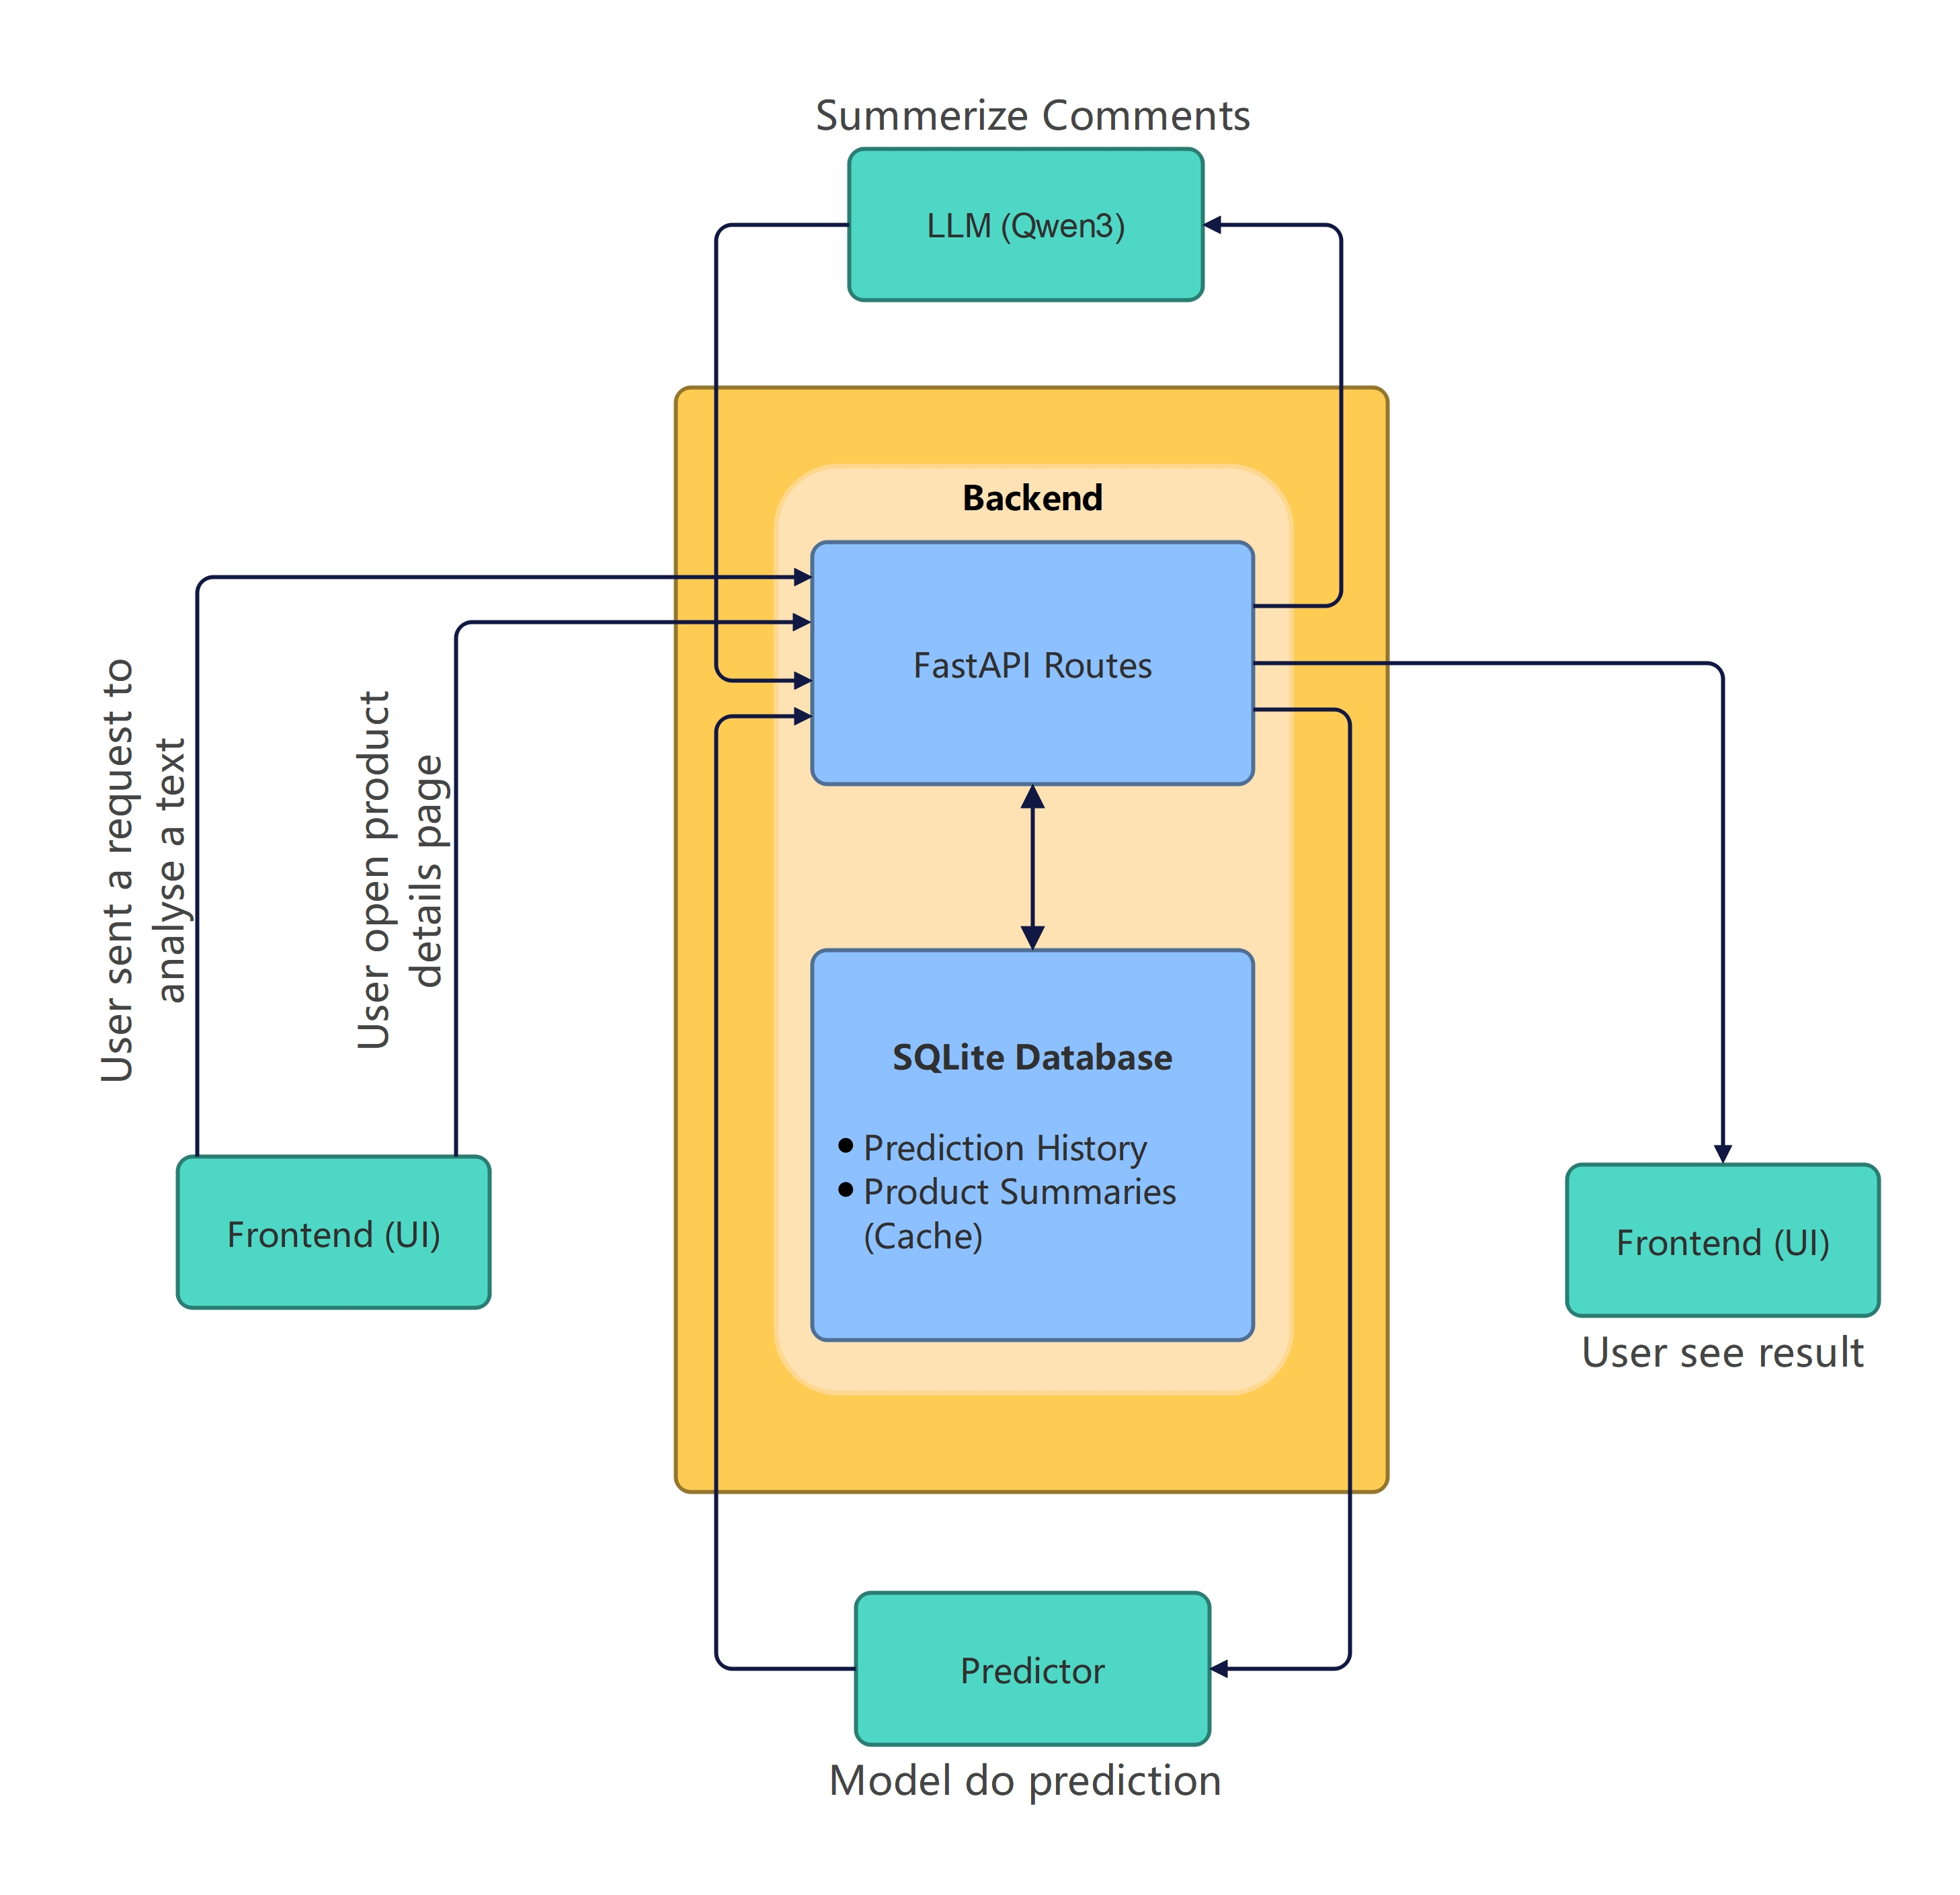
\includegraphics[width=1\textwidth]{figures/Drawing2.jpg}
	\caption{معماری بخش Backend و جریان پردازش درخواست‌ها}
	\label{fig:backendworkflow}
\end{figure}

\section{طراحی و پیاده‌سازی Frontend}
رابط کاربری (Frontend) این پروژه با استفاده از کتابخانه React و زبان TypeScript توسعه داده شده است. هدف از طراحی این بخش، ایجاد محیطی ساده، سریع و کاربرپسند برای برقراری ارتباط کاربران با سامانه تحلیل احساسات بوده است. کاربران از طریق این رابط می‌توانند محصولات را جستجو کنند، احساس نظرات را تحلیل نمایند، اطلاعات هر محصول را مشاهده کرده و نتایج پردازش مدل یادگیری ماشین را به‌صورت گرافیکی دریافت کنند.

در طراحی Frontend تلاش شده است تا علاوه بر زیبایی ظاهری، سرعت عملکرد، قابلیت توسعه و تجربه کاربری مناسب نیز در نظر گرفته شود. همچنین تمامی ارتباطات با Backend از طریق \lr{REST API} انجام شده و تمامی داده‌های نمایش داده‌شده در صفحات، به‌صورت پویا از سرور دریافت می‌شوند.
\subsection{معماری Frontend}
معماری پروژه بر اساس ساختار Component-Based در React طراحی شده است. در این معماری، رابط کاربری به مجموعه‌ای از کامپوننت‌های مستقل تقسیم شده است که هرکدام مسئول انجام وظیفه مشخصی هستند. این ساختار باعث افزایش خوانایی کد، قابلیت استفاده مجدد از کامپوننت‌ها و سهولت نگهداری پروژه می‌شود.

هر صفحه از سیستم از ترکیب چندین کامپوننت کوچک‌تر تشکیل شده است و تنها مسئول مدیریت منطق همان صفحه می‌باشد. همچنین ارتباط با Backend از طریق لایه مجزایی برای ارسال درخواست‌های HTTP انجام می‌شود که باعث کاهش وابستگی بین بخش‌های مختلف پروژه شده است.
\subsection{صفحات سیستم}
برای استفاده بهتر کاربران، رابط کاربری پروژه در قالب چند صفحه اصلی طراحی شده است. در ادامه تصاویری از بخش‌های رابط کاربری مشاهده می‌کنید:

\begin{figure}[H]
	\centering
	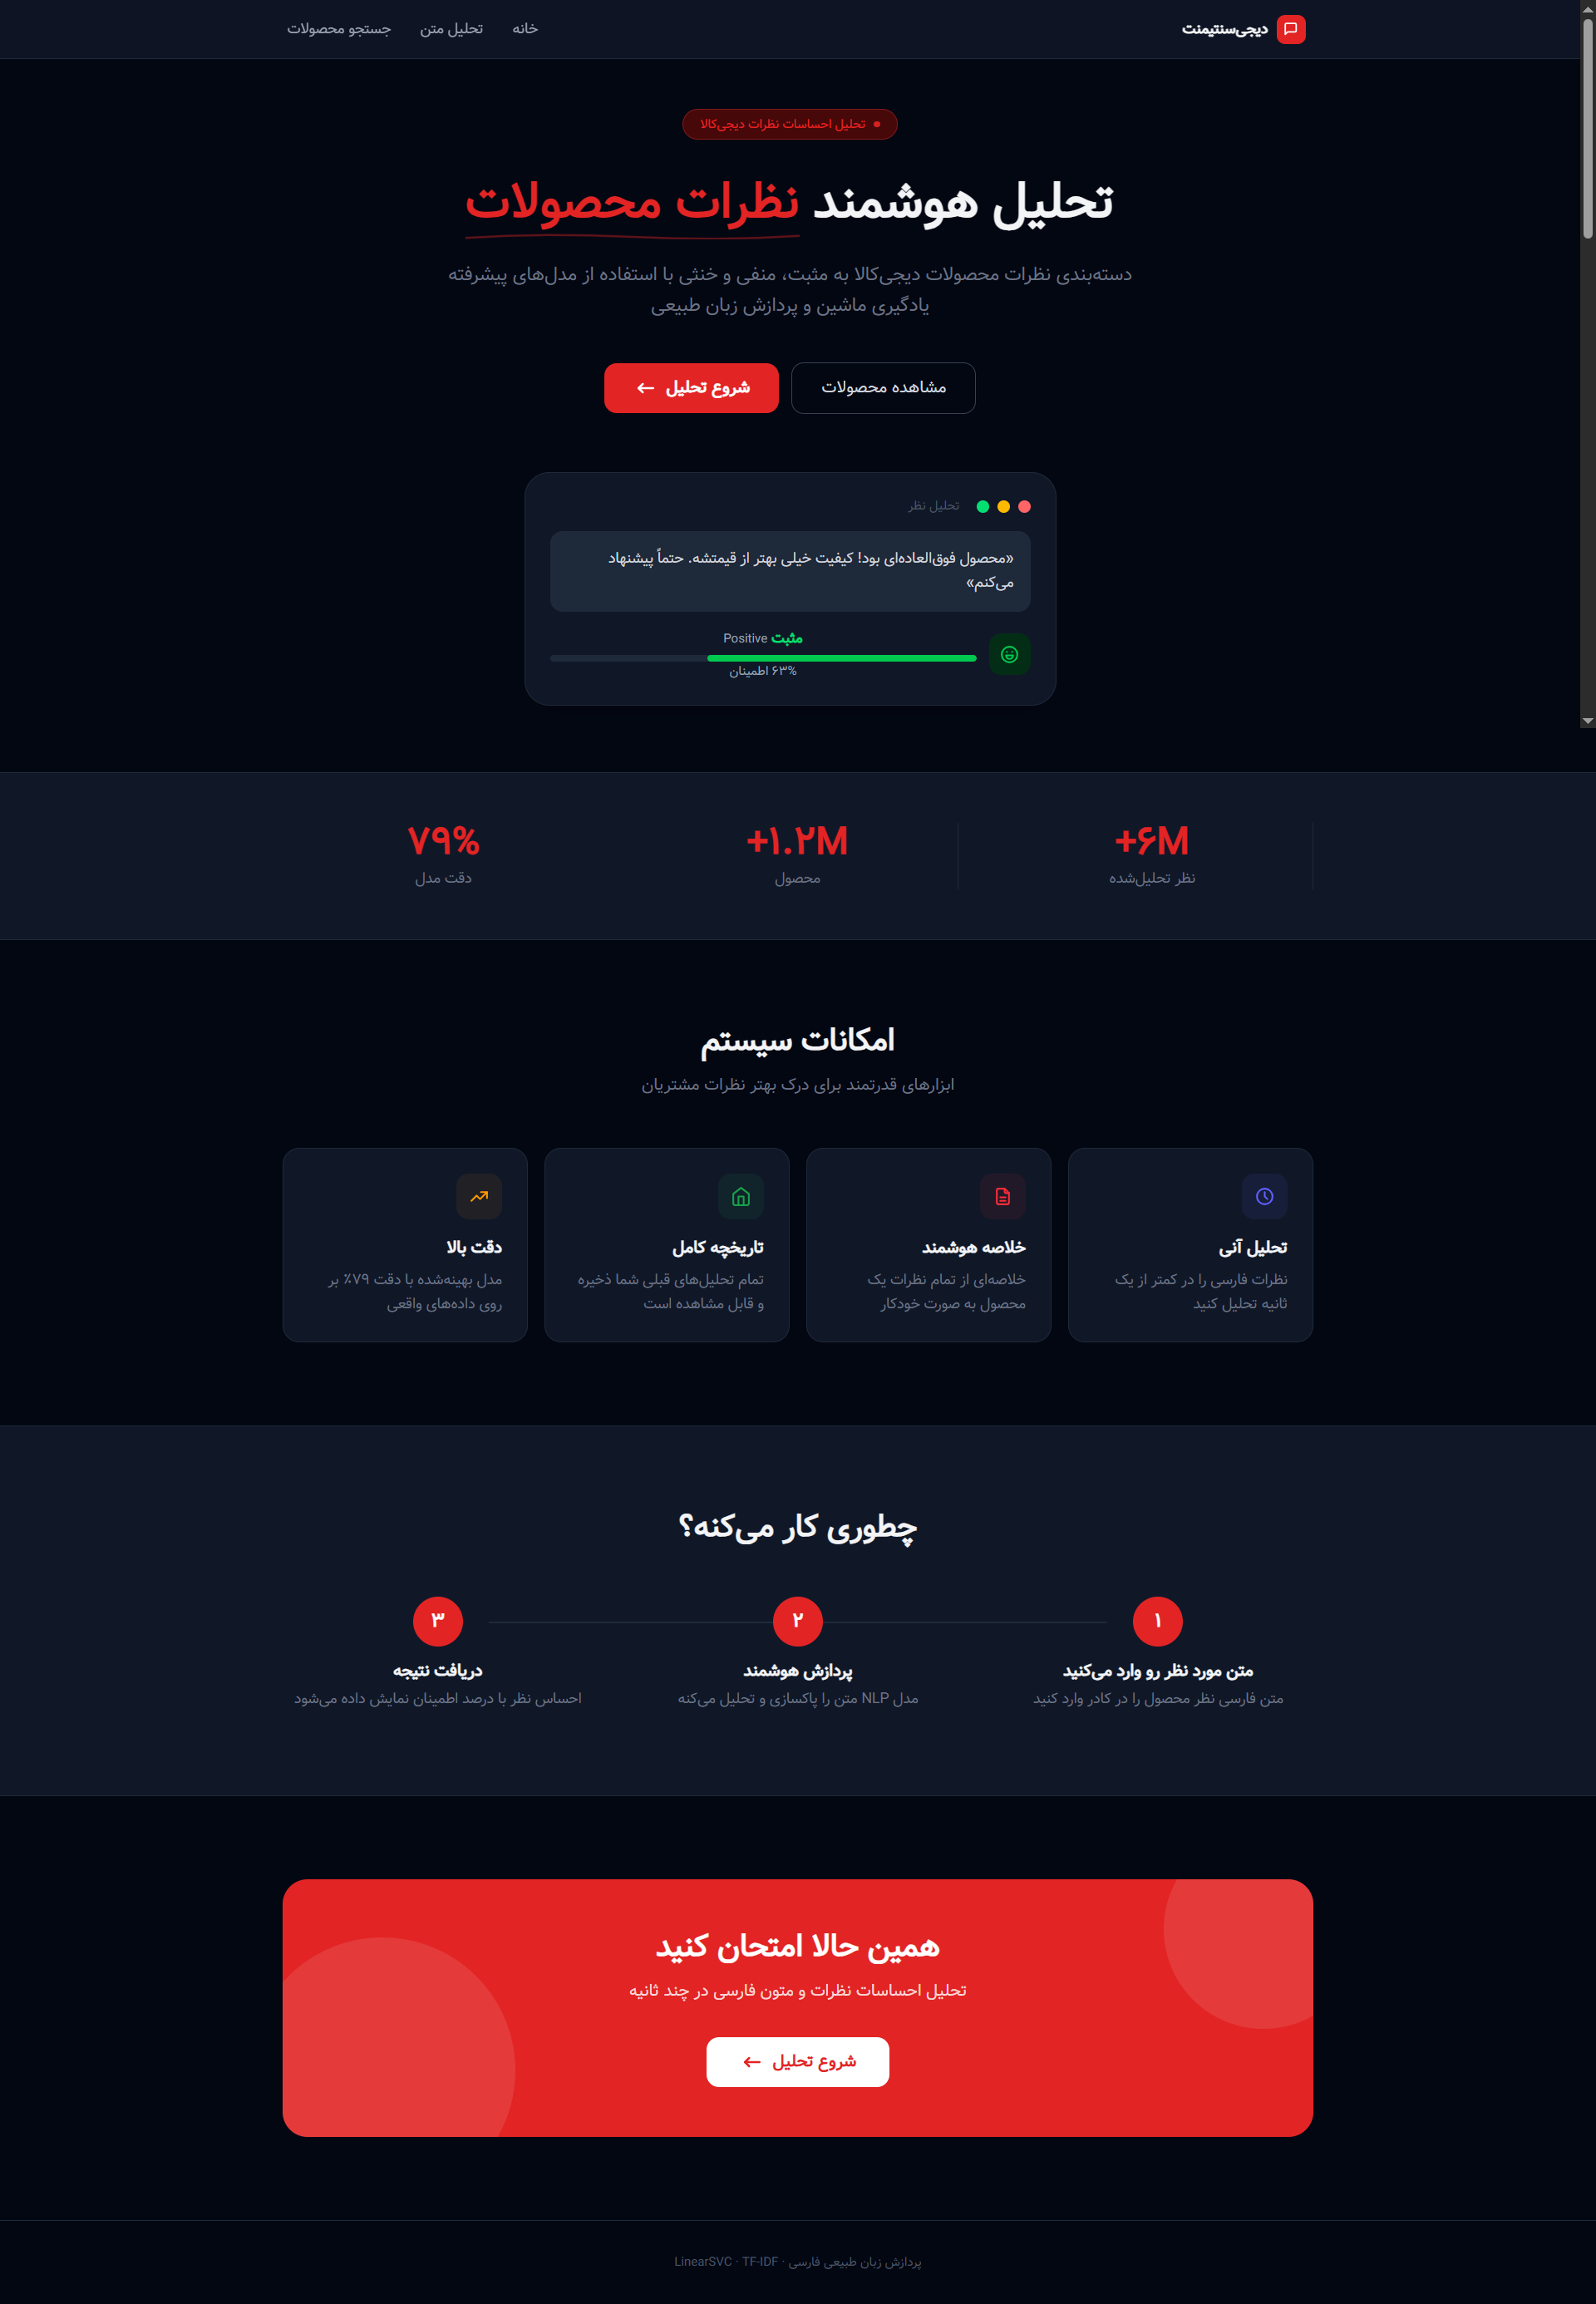
\includegraphics[width=0.8\textwidth]{figures/screen1.png}
	\caption{صفحه اصلی وب اپلیکیشن}
	\label{fig:landingpage}
\end{figure}

این صفحه اولین بخشی است که کاربر پس از ورود به سامانه مشاهده می‌کند. در این صفحه معرفی کوتاهی از پروژه، امکانات سامانه و راه‌های دسترسی به بخش‌های مختلف سیستم نمایش داده می‌شود.

\begin{figure}[H]
	\centering
	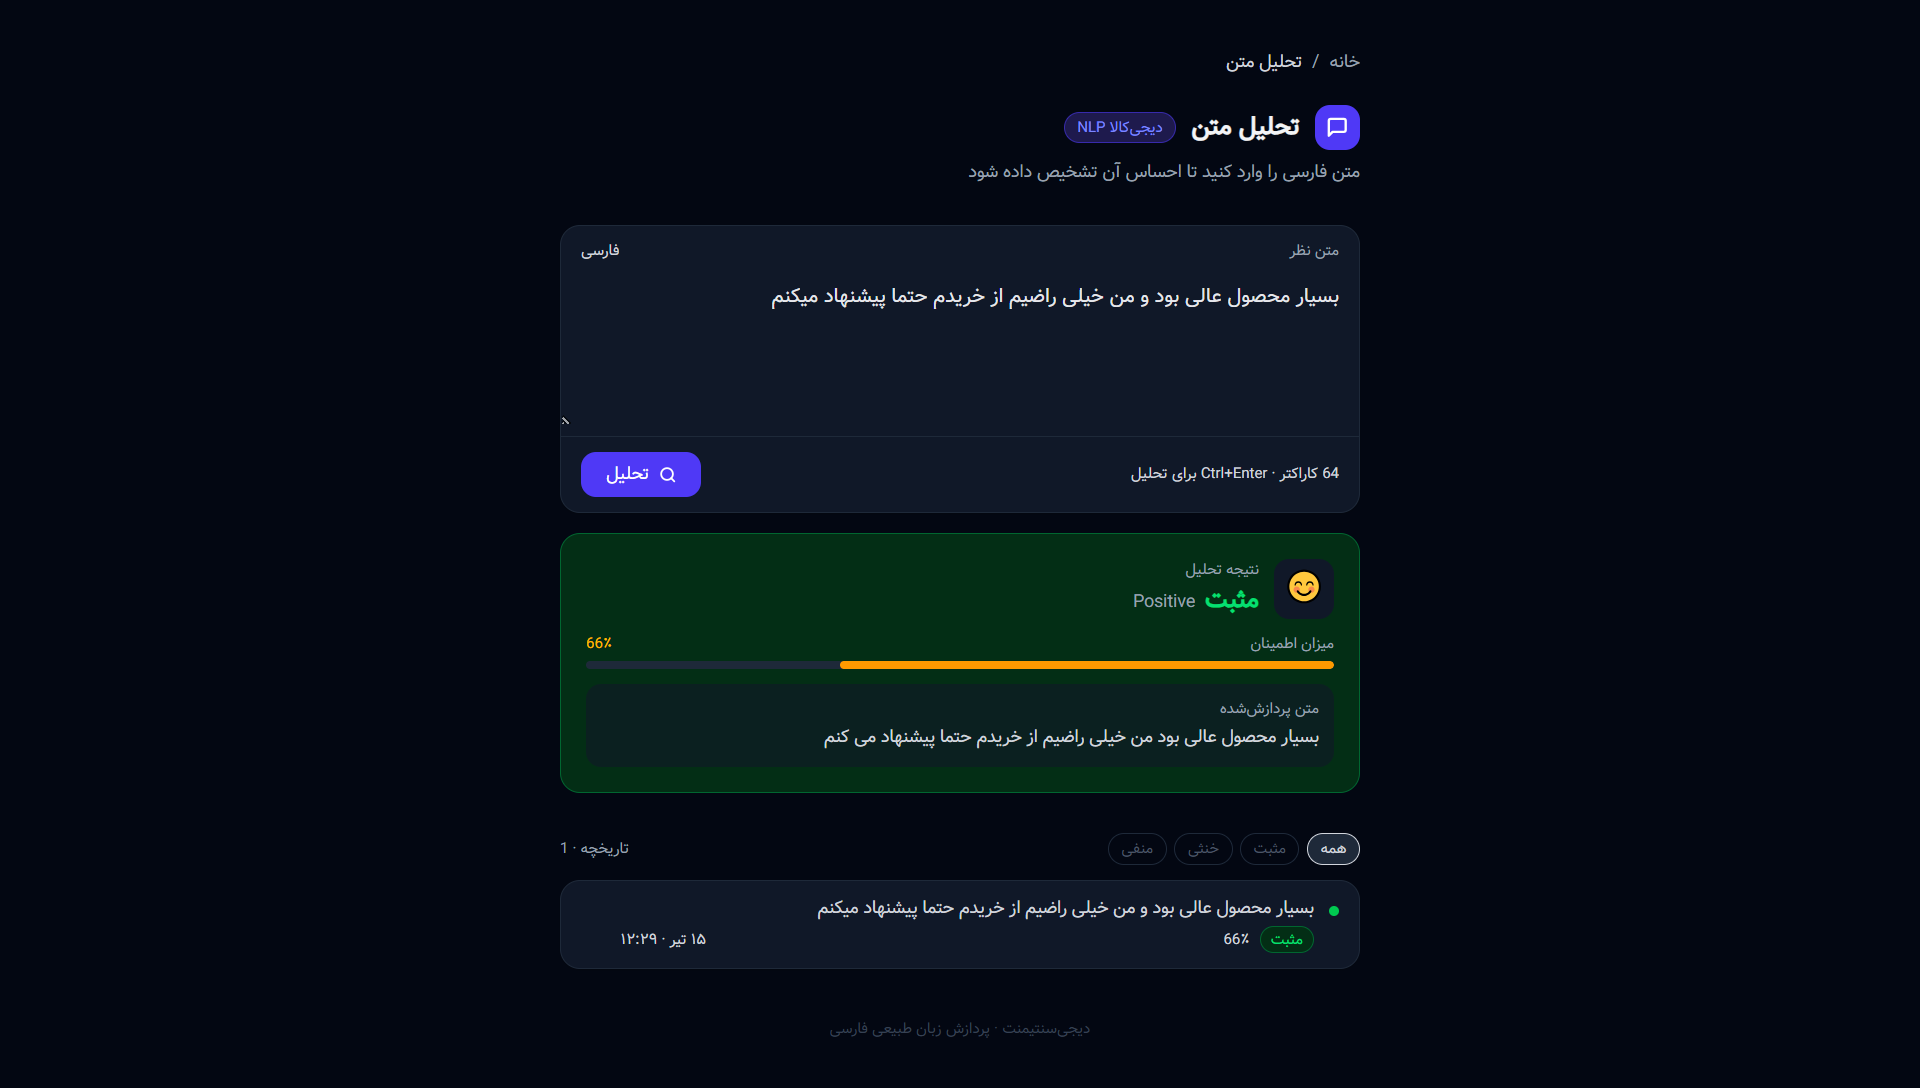
\includegraphics[width=1\textwidth]{figures/screen2.png}
	\caption{صفحه تحلیل احساسات (مثبت)}
	\label{fig:positivesentiment}
\end{figure}

\begin{figure}[H]
	\centering
	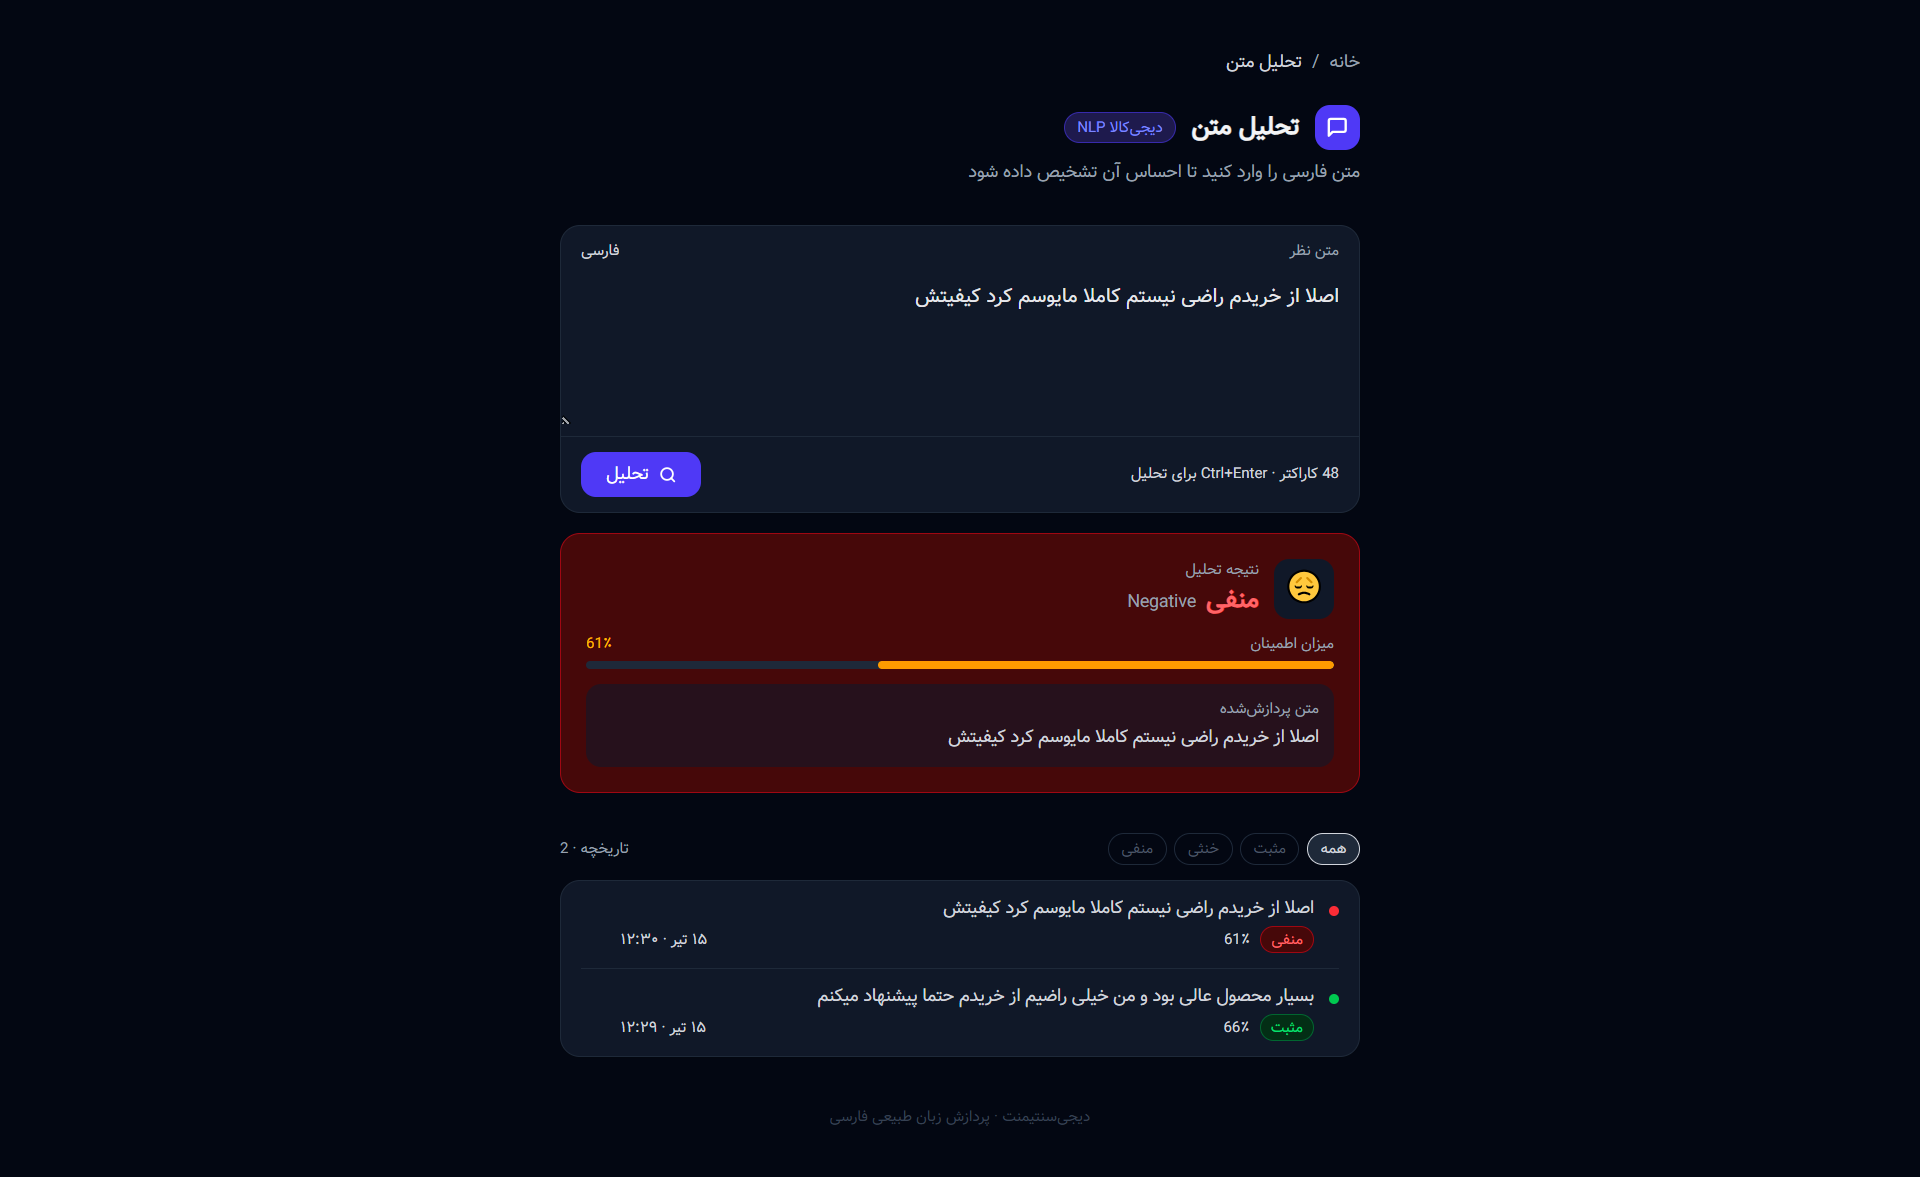
\includegraphics[width=1\textwidth]{figures/screen3.png}
	\caption{صفحه تحلیل احساسات (منفی)}
	\label{fig:negtivesentiment}
\end{figure}

\begin{figure}[H]
	\centering
	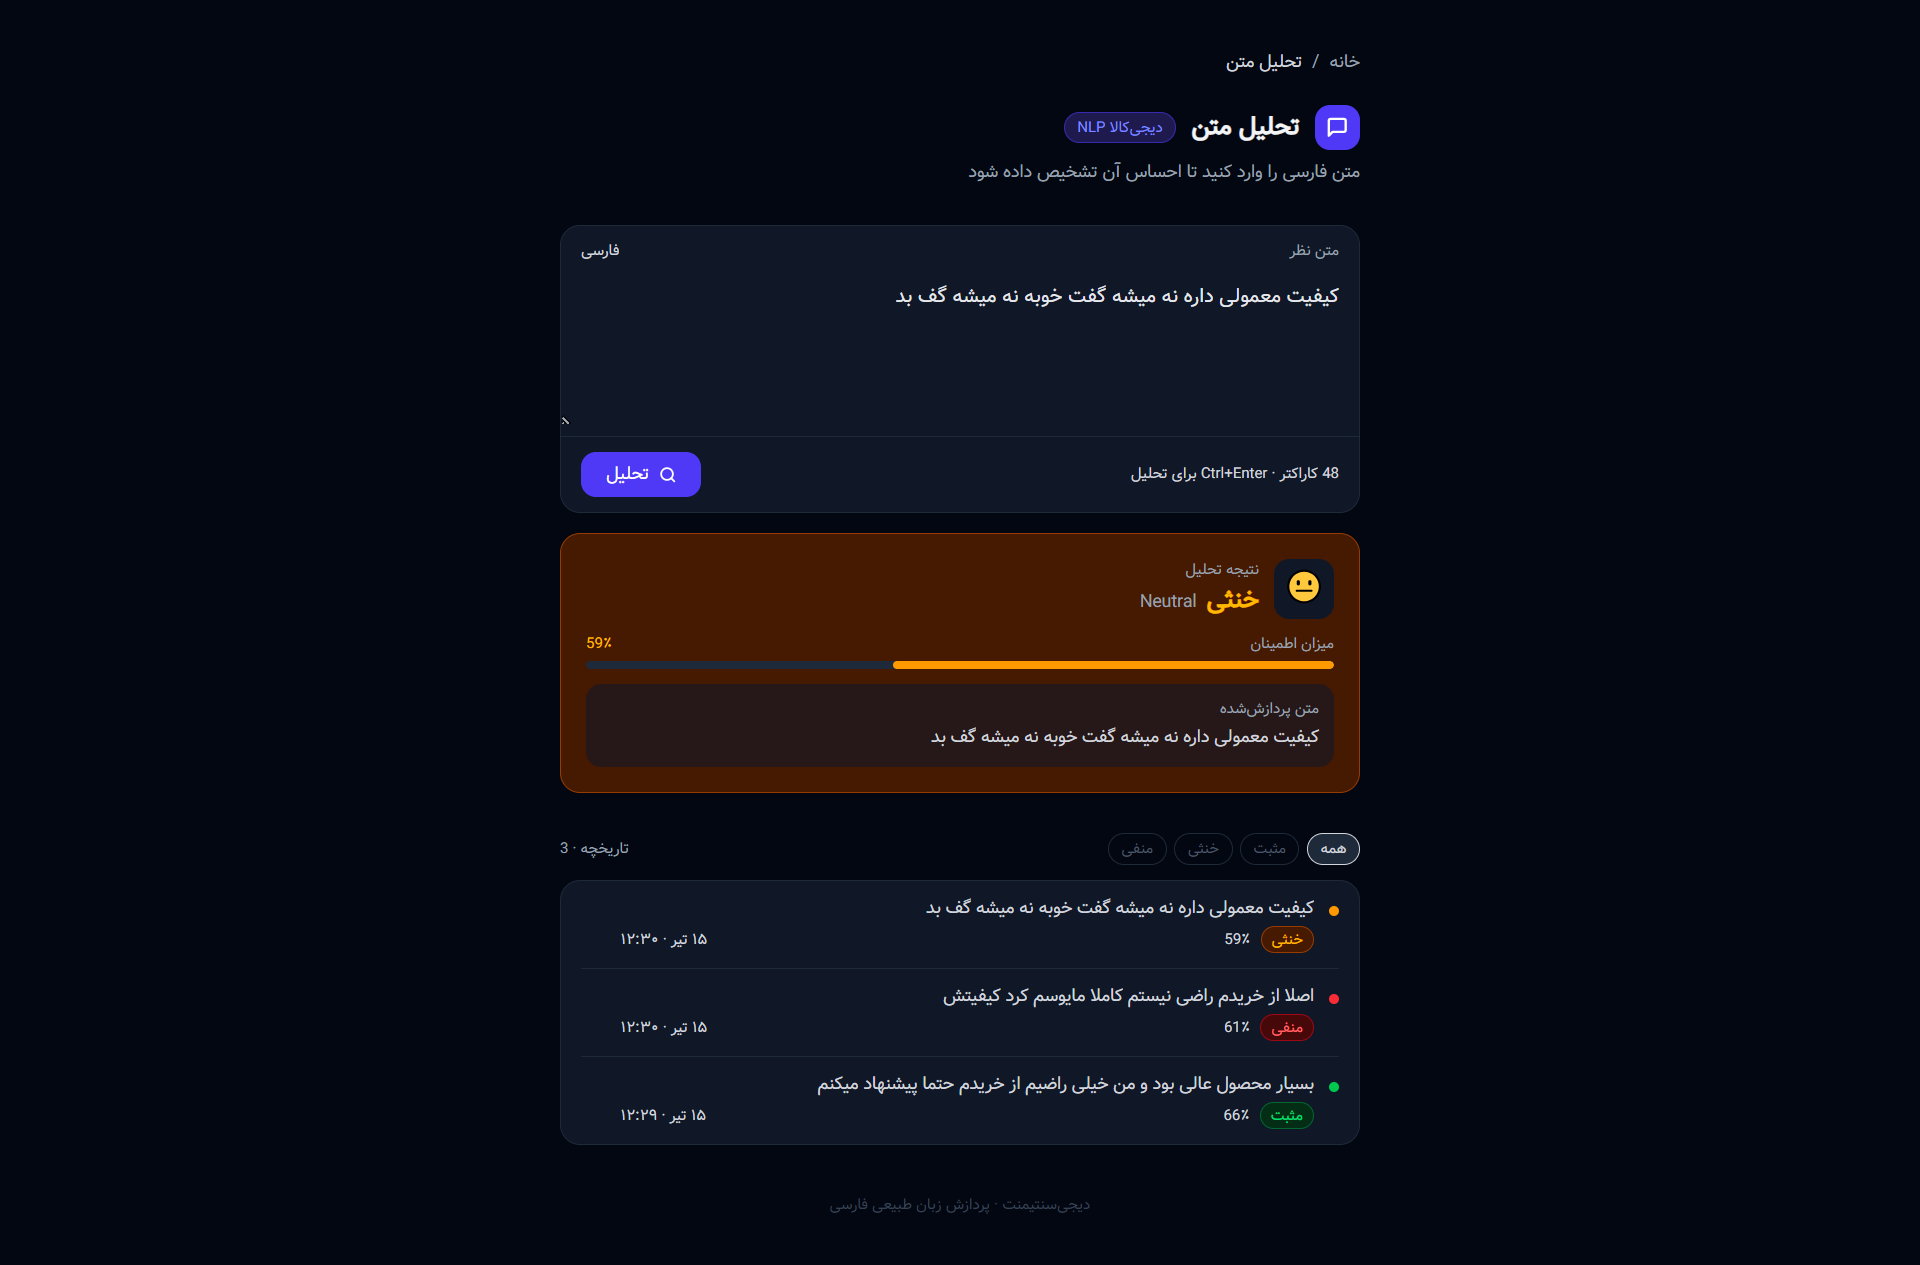
\includegraphics[width=1\textwidth]{figures/screen4.png}
	\caption{صفحه تحلیل احساسات (خنثی)}
	\label{fig:nutralsentiment}
\end{figure}

در این صفحه کاربر می‌تواند متن یک نظر را وارد کرده و پس از ارسال، نتیجه تحلیل احساسات را مشاهده کند. پس از دریافت پاسخ از Backend ، نوع احساس (مثبت، منفی یا خنثی)، میزان اطمینان مدل (Confidence) و سایر اطلاعات مرتبط به کاربر نمایش داده می‌شود.

\begin{figure}[H]
	\centering
	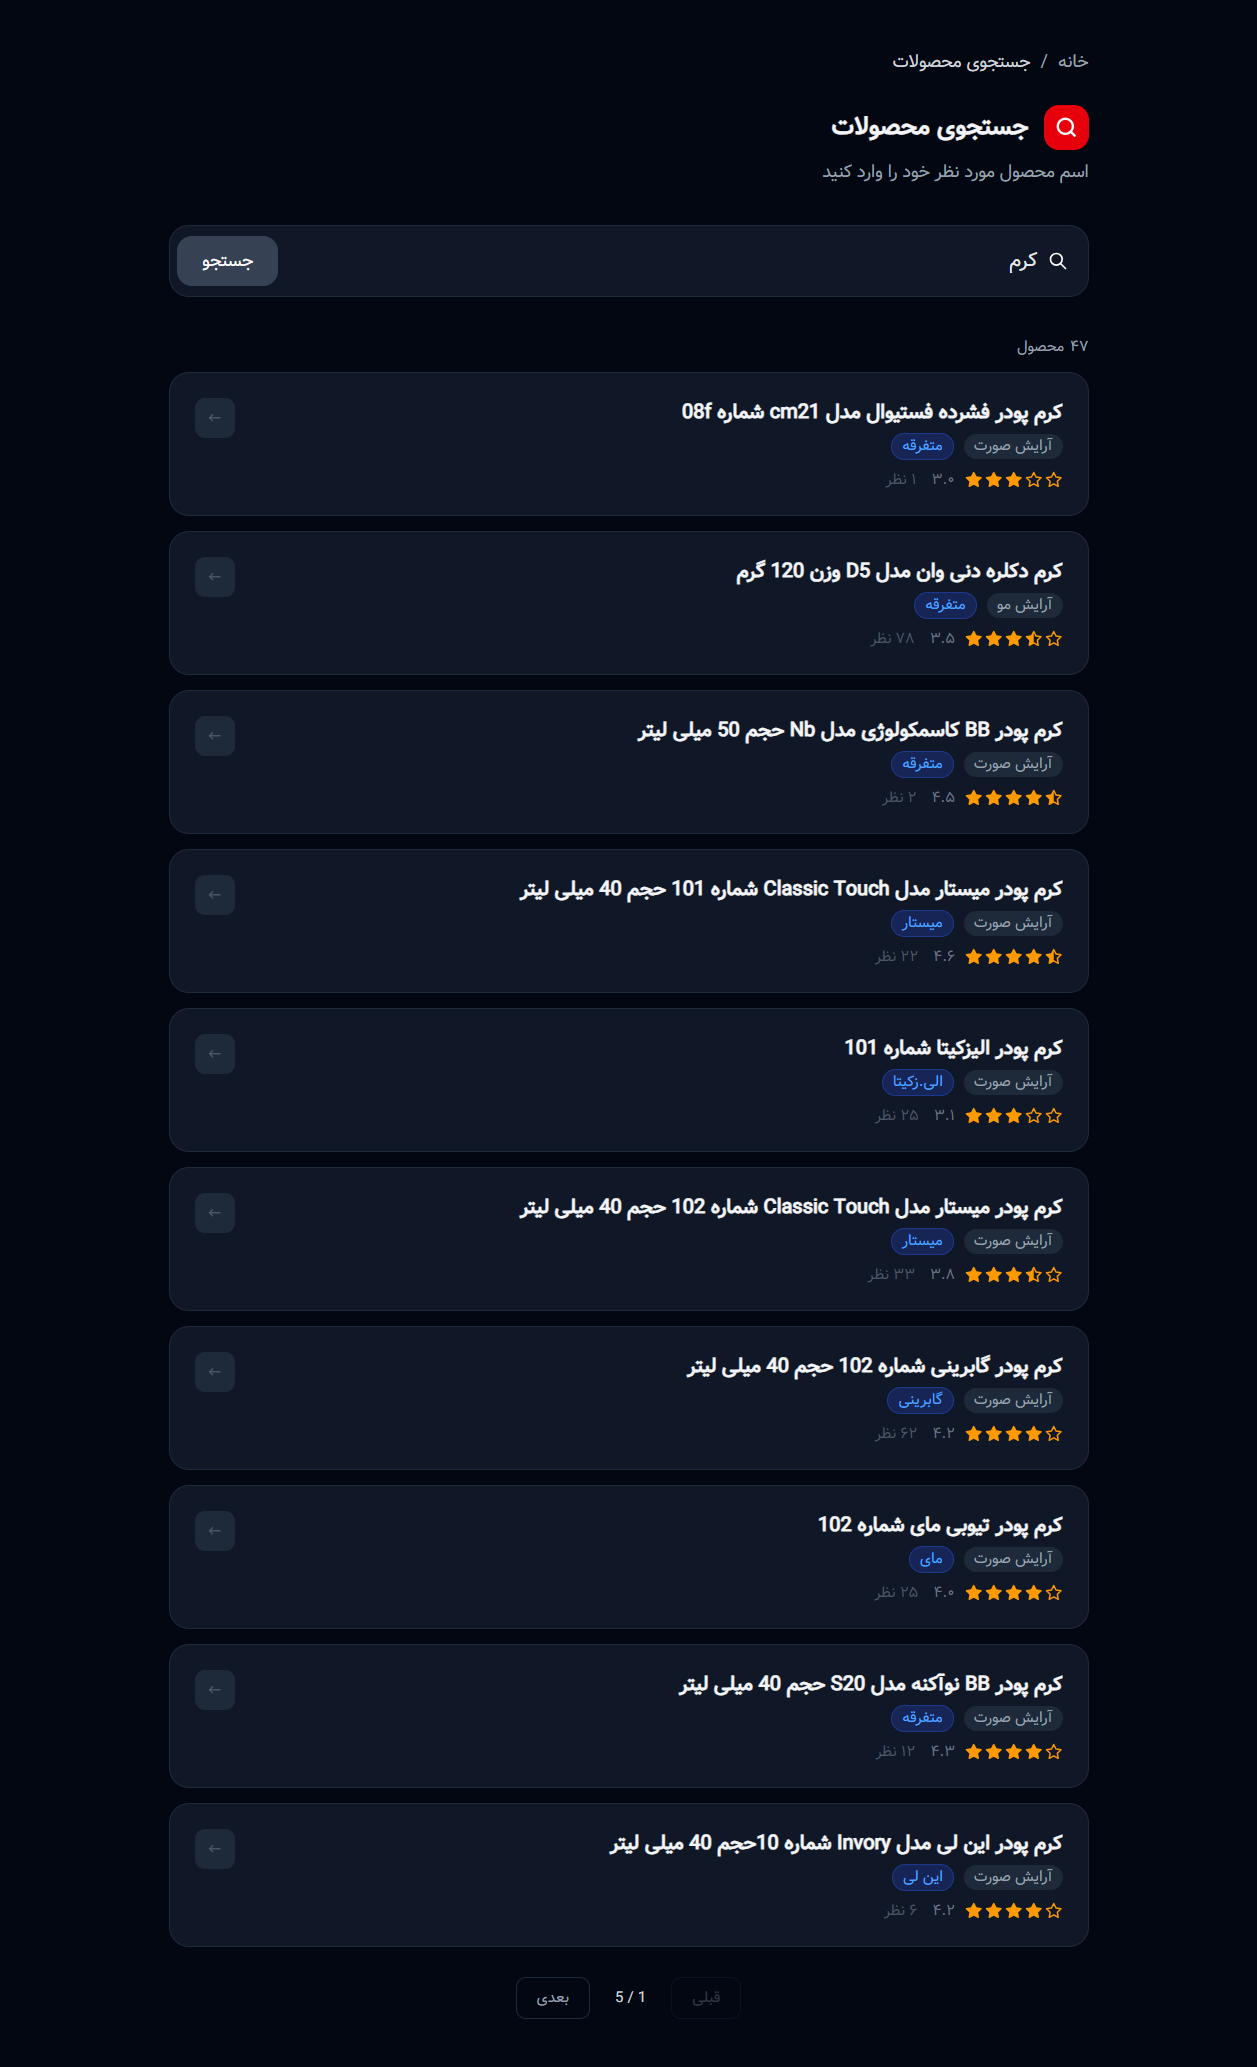
\includegraphics[width=0.7\textwidth]{figures/screen5.png}
	\caption{صفحه جستجوی محصولات}
	\label{fig:searchproducts}
\end{figure}

این صفحه امکان جستجوی محصولات را بر اساس نام، برند یا دسته‌بندی فراهم می‌کند. نتایج جستجو به‌صورت پویا از Backend دریافت شده و کاربران می‌توانند محصول موردنظر خود را انتخاب کنند.

\begin{figure}[H]
	\centering
	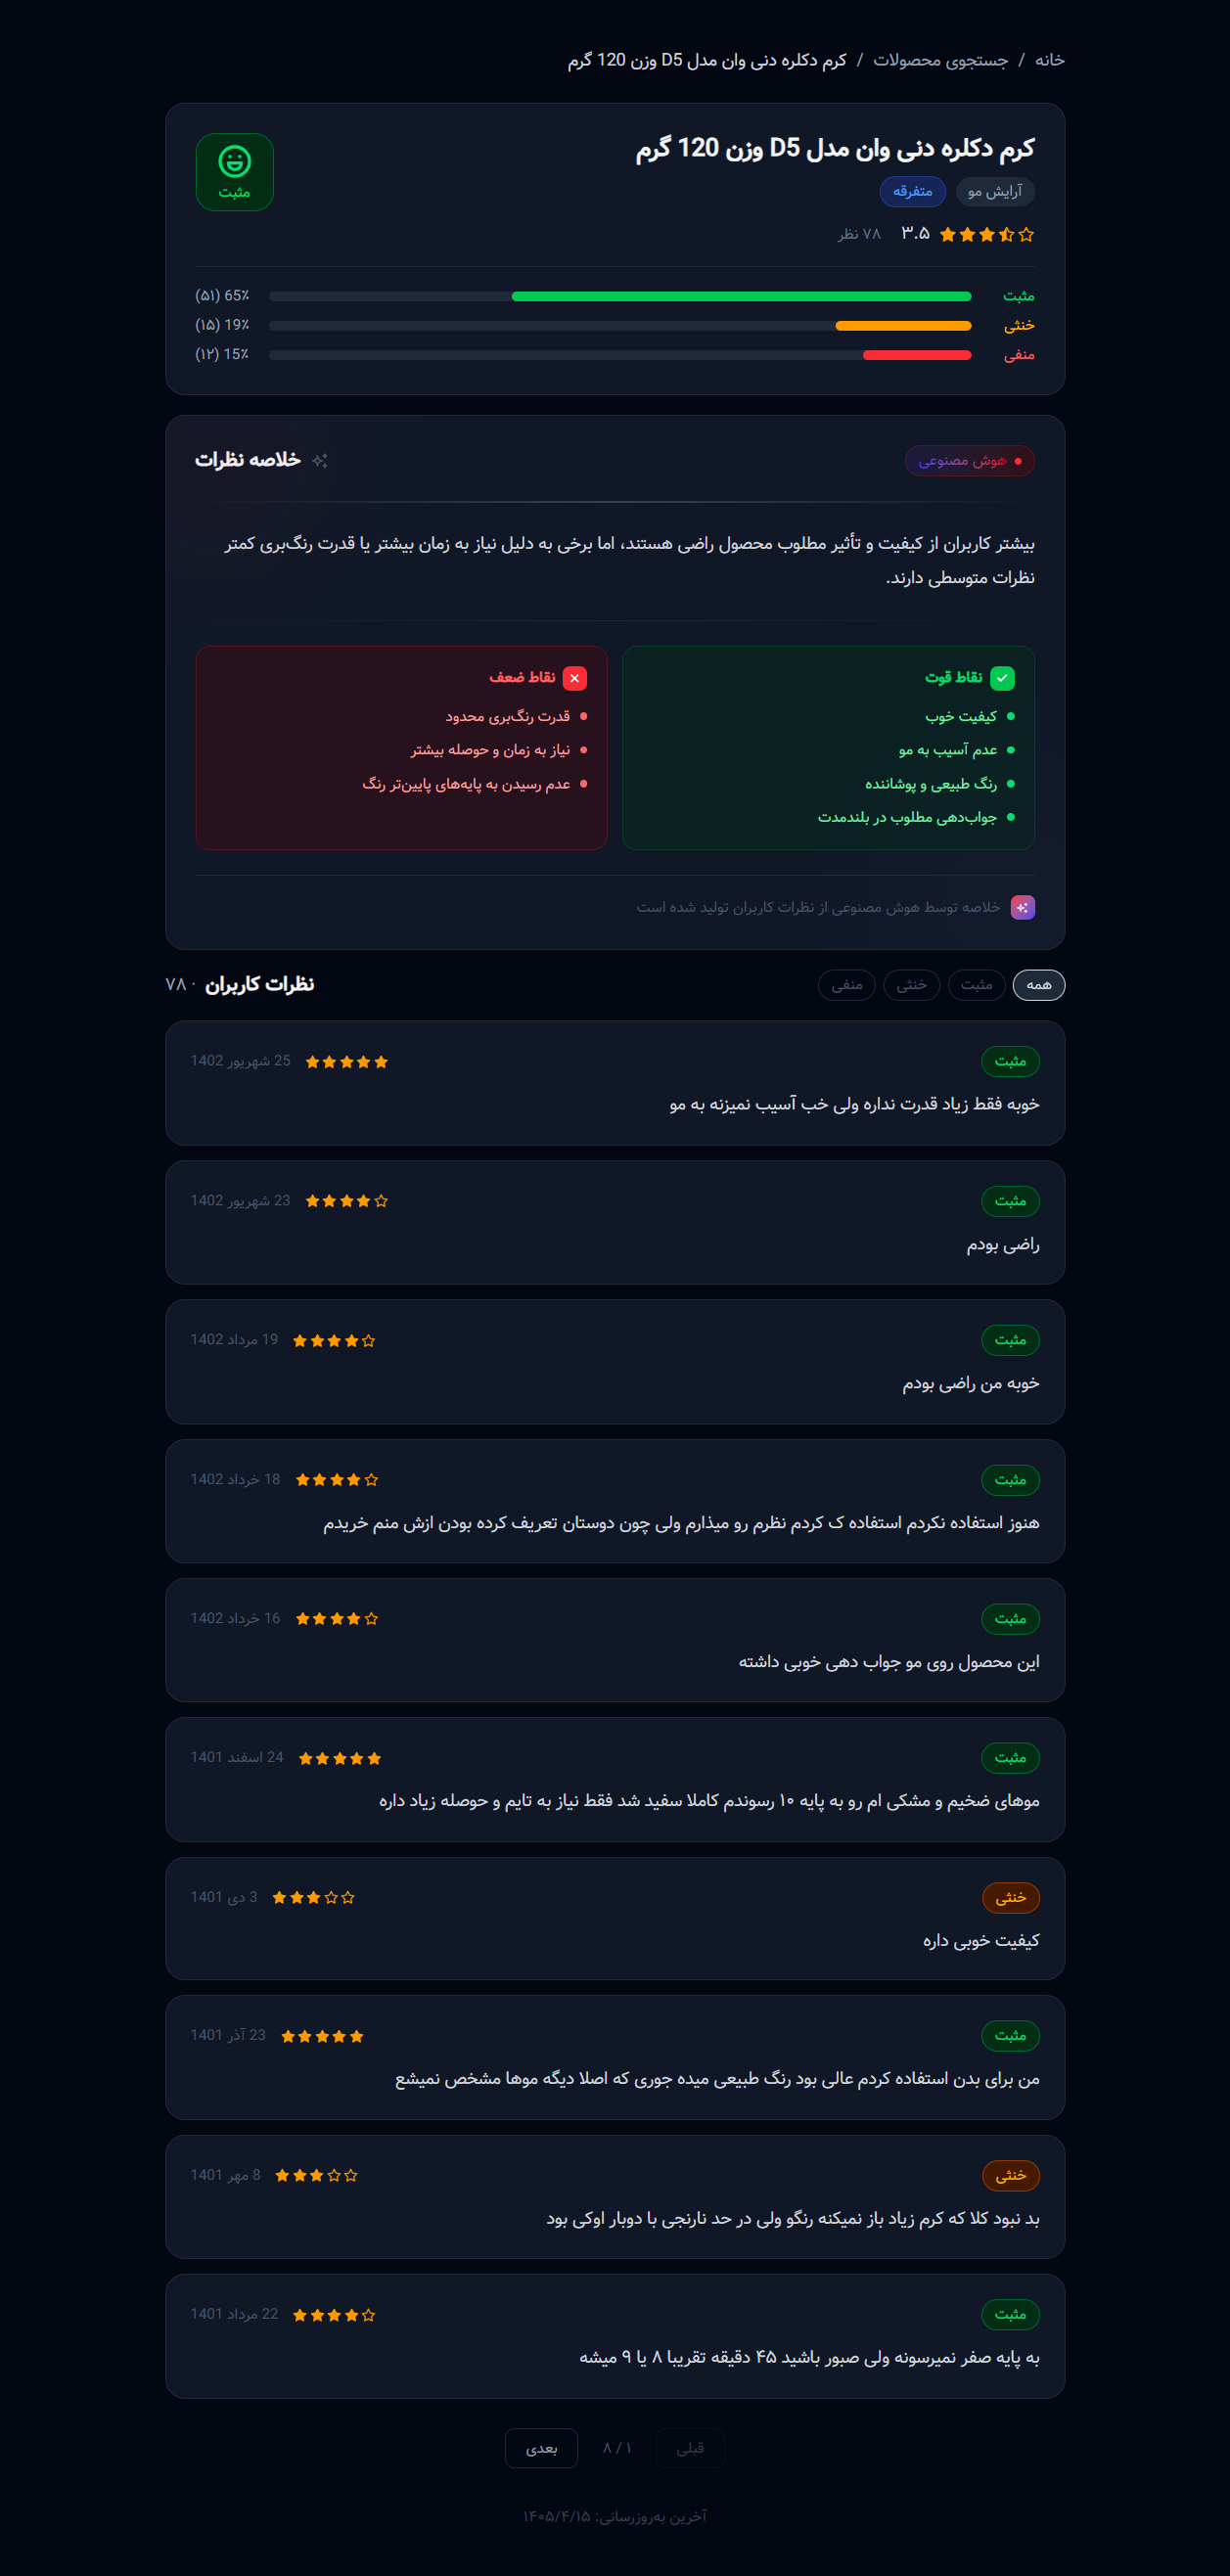
\includegraphics[width=0.7\textwidth, keepaspectratio]{figures/screen6.png}
	\caption{صفحه جزئیات محصول}
	\label{fig:productdetails}
\end{figure}

پس از انتخاب یک محصول، اطلاعات کامل آن نمایش داده می‌شود. این اطلاعات شامل مشخصات محصول، تعداد نظرات، توزیع احساسات کاربران، خلاصه نظرات تولیدشده توسط سیستم و فهرست نظرات ثبت‌شده برای محصول است. همچنین امکان مشاهده نظرات به‌صورت صفحه‌بندی‌شده نیز فراهم شده است.
\subsection{ارتباط با Backend}
تمامی ارتباطات Frontend با Backend از طریق Axios و سرویس‌های \lr{REST API} انجام می‌شود. برای هر عملیات، درخواست مناسب به سرور ارسال شده و پس از دریافت پاسخ، اطلاعات موردنیاز در رابط کاربری نمایش داده می‌شود.

از جمله مهم‌ترین درخواست‌های ارسال‌شده می‌توان به موارد زیر اشاره کرد:
\begin{itemize}
	\item ارسال متن برای تحلیل احساسات
	\item جستجوی محصولات
	\item دریافت اطلاعات کامل هر محصول
	\item دریافت خلاصه نظرات
	\item دریافت لیست نظرات محصولات
\end{itemize}
جداسازی منطق ارتباط با سرور در پوشه services باعث شده است که مدیریت API ها ساده‌تر شده و در صورت تغییر Backend ، تنها این بخش نیاز به بروزرسانی داشته باشد.
\subsection{مدیریت وضعیت برنامه \lr{(State Management)}}
برای مدیریت داده‌های مشترک میان صفحات مختلف از کتابخانه Zustand استفاده شده است. این کتابخانه نسبت به بسیاری از راهکارهای دیگر حجم کمتری داشته و پیاده‌سازی ساده‌تری ارائه می‌دهد.

اطلاعاتی مانند نتایج جستجو، داده‌های محصولات، وضعیت بارگذاری (Loading) ، اطلاعات تحلیل احساسات و سایر داده‌های مشترک در Store های برنامه نگهداری می‌شوند تا بدون نیاز به ارسال مکرر درخواست یا انتقال داده بین کامپوننت‌ها، در تمامی بخش‌های موردنیاز قابل استفاده باشند.
\subsection{طراحی رابط کاربری}
در طراحی رابط کاربری پروژه از \lr{Tailwind CSS } استفاده شده است. این فریم‌ورک امکان طراحی سریع، منظم و واکنش‌گرا را فراهم کرده است.

در طراحی صفحات، سادگی و تجربه کاربری مناسب در اولویت قرار گرفته است. استفاده از کارت‌های اطلاعاتی (Cards) ، دکمه‌های استاندارد، نمایش مناسب وضعیت بارگذاری، چیدمان منظم اطلاعات و طراحی واکنش‌گرا باعث شده است که کاربران بتوانند در دستگاه‌های مختلف از سامانه استفاده کنند.

\section{‌پیشنهادات آینده و دسترسی به کد منبع و مستندات}
\subsection{پیشنهادات برای توسعه آینده}
با توجه به ساختار ماژولار پروژه، قابلیت‌های متعددی می‌توانند در نسخه‌های آینده به آن اضافه شوند. برخی از مهم‌ترین پیشنهادها عبارت‌اند از:
\begin{itemize}
	\item استفاده از مدل‌های مبتنی بر Transformer مانند ParsBERT یا XLM-RoBERTa برای افزایش دقت تحلیل احساسات
	\item آموزش مدل روی کل مجموعه داده شش میلیون نظر کاربران
	\item استفاده از پایگاه داده PostgreSQL به‌جای SQLite برای افزایش مقیاس‌پذیری
	\item استقرار پروژه با استفاده از Docker و طراحی فرآیند CI/CD
	\item توسعه سیستم پیشنهاد محصول بر اساس تحلیل احساسات کاربران
	\item افزودن داشبوردهای آماری و نمودارهای تحلیلی برای مدیران
	\item پیاده‌سازی احراز هویت کاربران و ایجاد حساب کاربری
	\item توسعه نسخه موبایل یا تبدیل سامانه به یک برنامه \lr{Progressive Web App (PWA)}
\end{itemize}
در مجموع، نتایج این پروژه نشان می‌دهد که استفاده از روش‌های یادگیری ماشین در کنار طراحی مناسب نرم‌افزار می‌تواند سامانه‌ای کاربردی و قابل توسعه برای تحلیل احساسات متون فارسی ایجاد کند. همچنین ساختار پیاده‌سازی‌شده این پروژه، بستر مناسبی برای توسعه قابلیت‌های پیشرفته‌تر در آینده فراهم کرده و می‌تواند به‌عنوان پایه‌ای برای پروژه‌های پژوهشی و صنعتی در حوزه پردازش زبان طبیعی مورد استفاده قرار گیرد.

\subsection{دسترسی به کد منبع و مستندات}
\begin{itemize}
	\item \textbf{ریپازیتوری گیتهاب:}\\
	\url{https://github.com/ArefOrumiehei/digikala-prods-comments-analysis}
	
	\item \textbf{مستندات \lr{API (Swagger)}:}\\
	\begin{figure}[H]
		\centering
		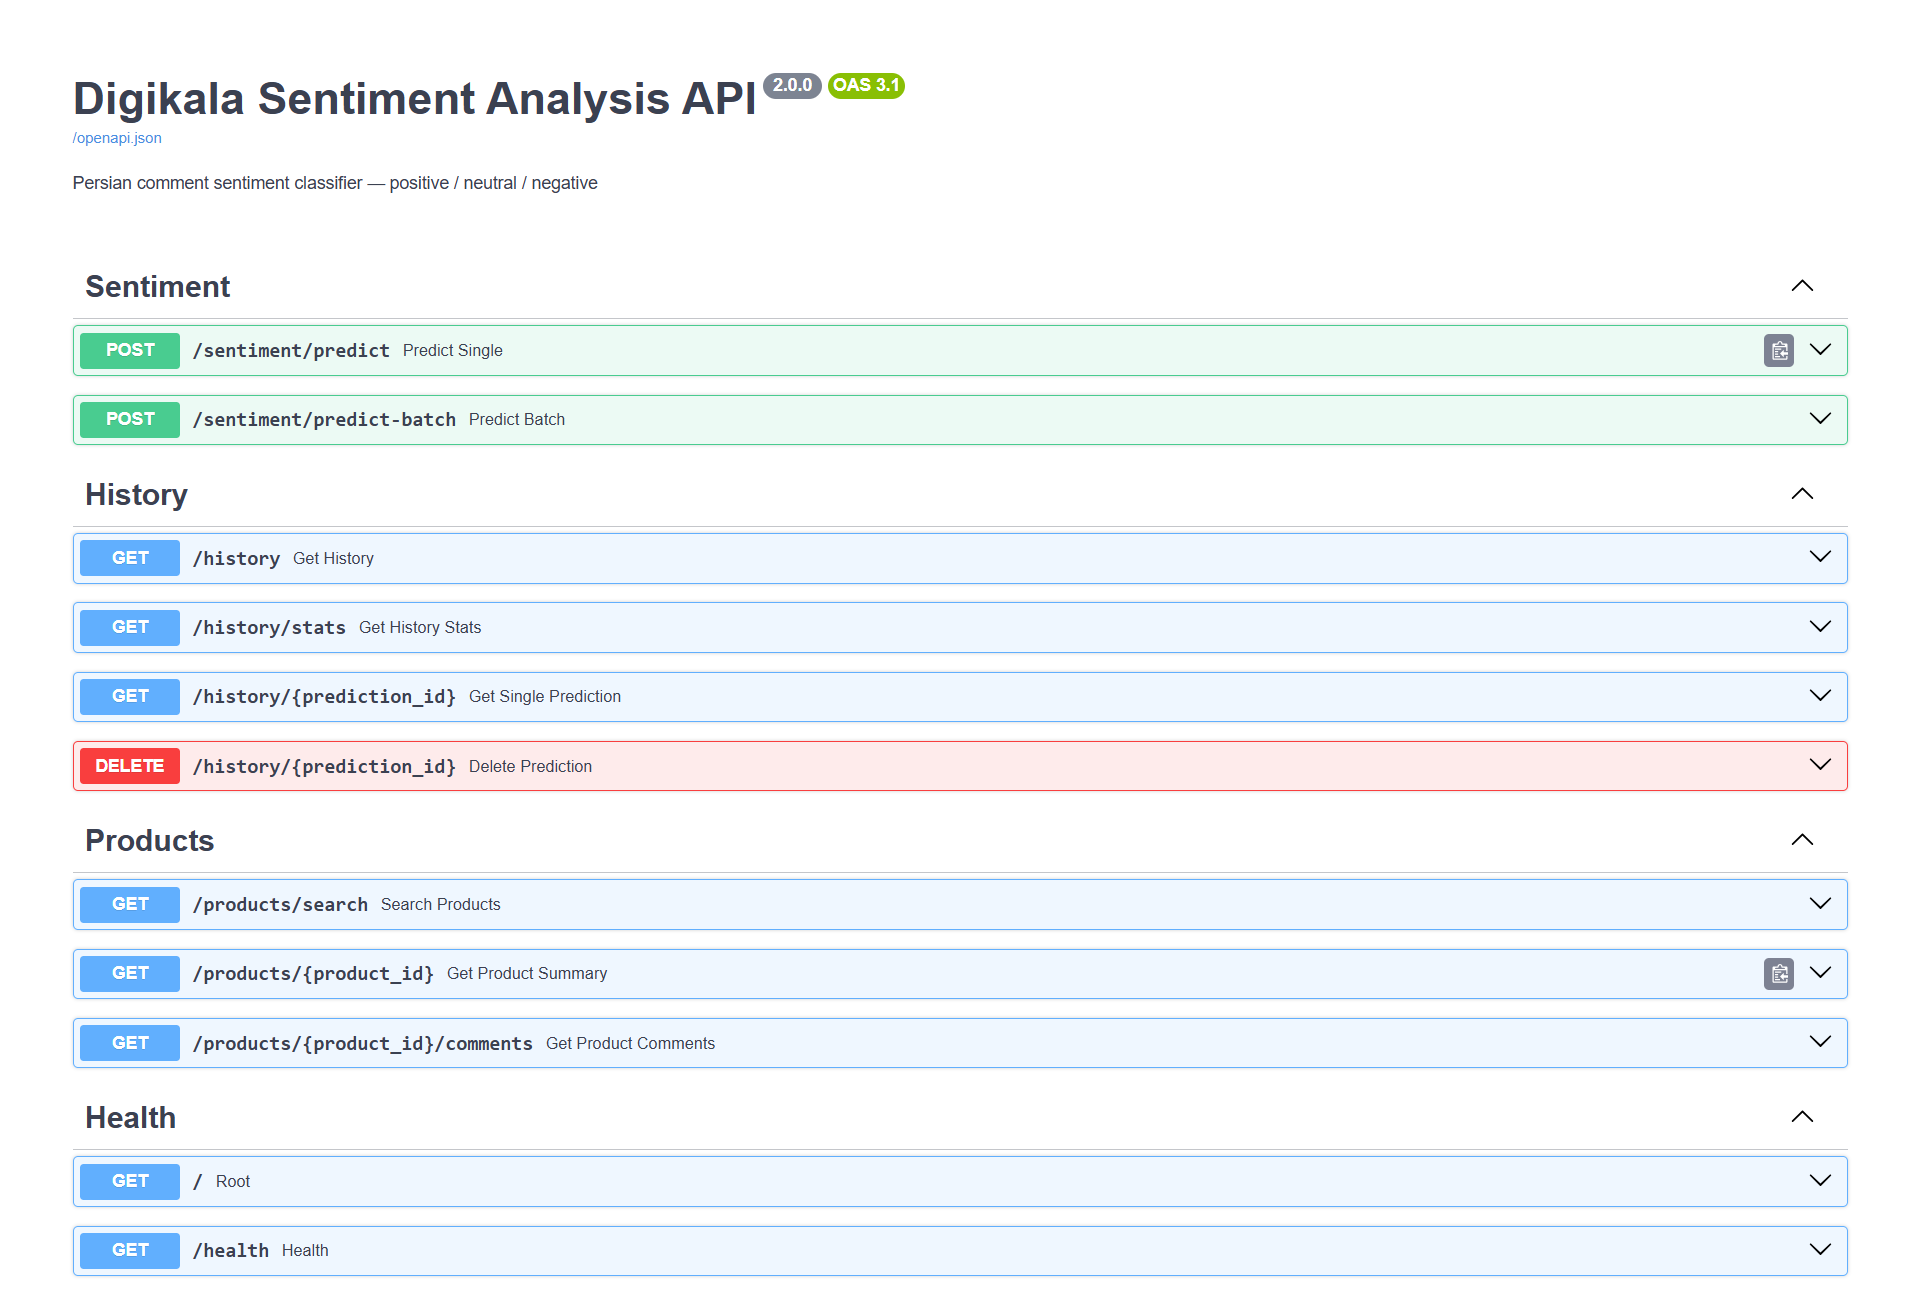
\includegraphics[width=1\textwidth]{figures/screen7.png}
		\caption{مستندات سرویس‌ها}
		\label{fig:swagger}
	\end{figure}
\end{itemize}



